\documentclass[leqno, openany]{memoir}
\setulmarginsandblock{3.5cm}{3.5cm}{*}
\setlrmarginsandblock{3cm}{3.5cm}{*}
\checkandfixthelayout

\usepackage{amsmath}
\usepackage{amssymb}
\usepackage{amsthm}
%\usepackage{MnSymbol}
\usepackage{bm}
\usepackage{accents}
\usepackage{mathtools}
\usepackage{tikz}
\usetikzlibrary{calc}
\usetikzlibrary{automata,positioning}
\usepackage{tikz-cd}
\usepackage{forest}
\usepackage{braket} 
\usepackage{listings}
\usepackage{mdframed}
\usepackage{verbatim}
\usepackage{physics}
\usepackage{ytableau}
\usepackage{caption}
\usepackage{subcaption}
\usepackage{dynkin-diagrams}
\usepackage{rank-2-roots}
\usepackage{stmaryrd}
\usepackage{stackengine}

%font
\usepackage[sc]{mathpazo}
\usepackage{eulervm}
\usepackage{berasans}
\usepackage{inconsolata}
%\usepackage{tgpagella}
\usepackage{microtype}

%CS packages
\usepackage{algorithmicx}
\usepackage{algpseudocode}
\usepackage{algorithm}

% typeset and bib
\usepackage[english]{babel} 
\usepackage[utf8]{inputenc} 
\usepackage[T1]{fontenc} 
\usepackage[backend=biber, style=alphabetic]{biblatex}
\usepackage[bookmarks, colorlinks, breaklinks]{hyperref} 
\hypersetup{linkcolor=black,citecolor=black,filecolor=black,urlcolor=black}

% other formatting packages
\usepackage{float}
\usepackage{booktabs}
\usepackage{enumitem}
\usepackage{csquotes}
\usepackage{titlesec}
\usepackage{titling}
\usepackage{fancyhdr}
\usepackage{lastpage}
\usepackage{parskip}

\usepackage{lipsum}

% delimiters
\DeclarePairedDelimiter{\gen}{\langle}{\rangle}
\DeclarePairedDelimiter{\floor}{\lfloor}{\rfloor}
\DeclarePairedDelimiter{\ceil}{\lceil}{\rceil}


\newtheorem{thm}{Theorem}[section]
\newtheorem{cor}[thm]{Corollary}
\newtheorem{prop}[thm]{Proposition}
\newtheorem{lem}[thm]{Lemma}
\newtheorem{conj}[thm]{Conjecture}
\newtheorem{quest}[thm]{Question}

\theoremstyle{definition}
\newtheorem{defn}[thm]{Definition}
\newtheorem{defns}[thm]{Definitions}
\newtheorem{con}[thm]{Construction}
\newtheorem{exm}[thm]{Example}
\newtheorem{exms}[thm]{Examples}
\newtheorem{notn}[thm]{Notation}
\newtheorem{notns}[thm]{Notations}
\newtheorem{addm}[thm]{Addendum}
\newtheorem{exer}[thm]{Exercise}

\theoremstyle{remark}
\newtheorem{rmk}[thm]{Remark}
\newtheorem{rmks}[thm]{Remarks}
\newtheorem{warn}[thm]{Warning}
\newtheorem{sch}[thm]{Scholium}


% unnumbered theorems
\theoremstyle{plain}
\newtheorem*{thm*}{Theorem}
\newtheorem*{prop*}{Proposition}
\newtheorem*{lem*}{Lemma}
\newtheorem*{cor*}{Corollary}
\newtheorem*{conj*}{Conjecture}

% unnumbered definitions
\theoremstyle{definition}
\newtheorem*{defn*}{Definition}
\newtheorem*{exer*}{Exercise}
\newtheorem*{defns*}{Definitions}
\newtheorem*{con*}{Construction}
\newtheorem*{exm*}{Example}
\newtheorem*{exms*}{Examples}
\newtheorem*{notn*}{Notation}
\newtheorem*{notns*}{Notations}
\newtheorem*{addm*}{Addendum}


\theoremstyle{remark}
\newtheorem*{rmk*}{Remark}

% shortcuts
\newcommand{\Ima}{\mathrm{Im}}
\newcommand{\A}{\mathbb{A}}
\newcommand{\F}{\mathbb{F}}
\newcommand{\N}{\mathbb{N}}
\newcommand{\R}{\mathbb{R}}
\newcommand{\C}{\mathbb{C}}
\renewcommand{\H}{\mathbb{H}}
\newcommand{\Z}{\mathbb{Z}}
\newcommand{\Q}{\mathbb{Q}}
\newcommand{\E}{\mathbb{E}}
\newcommand{\G}{\mathbb{G}}
\renewcommand{\k}{\Bbbk}
\renewcommand{\P}{\mathbb{P}}
\newcommand{\M}{\overline{M}}
\newcommand{\g}{\mathfrak{g}}
\newcommand{\h}{\mathfrak{h}}
\newcommand{\n}{\mathfrak{n}}
\renewcommand{\b}{\mathfrak{b}}
\newcommand{\ep}{\varepsilon}
\newcommand*{\dt}[1]{%
   \accentset{\mbox{\Huge\bfseries .}}{#1}}
\renewcommand{\abstractname}{Official Description}
\newcommand{\mc}[1]{\mathcal{#1}}
\newcommand{\T}{\mathbb{T}}
\newcommand{\mf}[1]{\mathfrak{#1}}
\newcommand{\mr}[1]{\mathrm{#1}}
\newcommand{\ms}[1]{\mathsf{#1}}
\newcommand{\ol}[1]{\overline{#1}}
\newcommand{\wtl}[1]{\widetilde{#1}}
\newcommand{\wh}[1]{\widehat{#1}}

\DeclareMathOperator{\Der}{Der}
\DeclareMathOperator{\Hom}{Hom}
\DeclareMathOperator{\End}{End}
\DeclareMathOperator{\ad}{ad}
\DeclareMathOperator{\Ad}{Ad}
\DeclareMathOperator{\Pic}{Pic}
\DeclareMathOperator{\Aut}{Aut}
\DeclareMathOperator{\Rad}{Rad}
\DeclareMathOperator{\supp}{supp}
\DeclareMathOperator{\sgn}{sgn}
\DeclareMathOperator{\spec}{Spec}
\DeclareMathOperator{\Spec}{Spec}
\DeclareMathOperator{\Proj}{Proj}
\DeclareMathOperator{\Lie}{\mathsf{Lie}}
\DeclareMathOperator{\Rep}{\mathsf{Rep}}
\DeclareMathOperator{\Mod}{\mathsf{Mod}}
\DeclareMathOperator{\chr}{char}
\DeclareMathOperator{\rk}{rk}

% Section formatting
\titleformat{\section}
    {\Large\sffamily\scshape\bfseries}{\thesection}{1em}{}
\titleformat{\subsection}[runin]
    {\large\sffamily\bfseries}{\thesubsection}{1em}{}
\titleformat{\subsubsection}[runin]{\normalfont\itshape}{\thesubsubsection}{1em}{}

\title{COURSE TITLE}
\author{Lectures by INSTRUCTOR, Notes by NOTETAKER}
\date{SEMESTER}

\newcommand*{\titleSW}
    {\begingroup% Story of Writing
    \raggedleft
    \vspace*{\baselineskip}
    {\Huge\itshape Lie Groups and Representations \\ Spring 2021}\\[\baselineskip]
    {\large\itshape Notes by Patrick Lei}\\[0.2\textheight]
    {\Large Lectures by Andrei Okounkov}\par
    \vfill
    {\Large \sffamily Columbia University}
    \vspace*{\baselineskip}
\endgroup}
\pagestyle{simple}

\chapterstyle{ell}


%\renewcommand{\cftchapterpagefont}{}
\renewcommand\cftchapterfont{\sffamily}
\renewcommand\cftsectionfont{\scshape}
\renewcommand*{\cftchapterleader}{}
\renewcommand*{\cftsectionleader}{}
\renewcommand*{\cftsubsectionleader}{}
\renewcommand*{\cftchapterformatpnum}[1]{~\textbullet~#1}
\renewcommand*{\cftsectionformatpnum}[1]{~\textbullet~#1}
\renewcommand*{\cftsubsectionformatpnum}[1]{~\textbullet~#1}
\renewcommand{\cftchapterafterpnum}{\cftparfillskip}
\renewcommand{\cftsectionafterpnum}{\cftparfillskip}
\renewcommand{\cftsubsectionafterpnum}{\cftparfillskip}
\setrmarg{3.55em plus 1fil}
\setsecnumdepth{subsection}
\maxsecnumdepth{subsection}
\settocdepth{subsection}

\begin{document}
    
\begin{titlingpage}
\titleSW
\end{titlingpage}

\thispagestyle{empty}
\section*{Disclaimer}%
\label{sec:disclaimer}

These notes were taken during lecture using the \texttt{vimtex} package of the
editor \texttt{neovim}.  Any errors are mine and not the instructor's.  In
addition, my notes are picture-free (but will include commutative diagrams) and
are a mix of my mathematical style and that of the instructor.  If you find any
errors, please contact me at \texttt{plei@math.columbia.edu}.  \newpage

\tableofcontents

\chapter{Lie algebras and algebraic groups}%
\label{cha:semisimple_lie_algebras}

If $G$ is a compact Lie group, then $\mf{g} = \ms{Lie}(G)$ has an invariant
metric $(-,-)$. If $\mf{g}_1 \subset \mf{g}$ is an ideal, then
$\mf{g}_1^{\perp}$ is also an ideal and we have $\mf{g} = \mf{g}_1 \oplus
\mf{g}_2$. In particular, we have \[ \mf{g} = \bigoplus \mf{g}_i \qquad
    \mf{g}_i = \begin{cases} \R \\ \text{simple nonabelian Lie algebra}
    \end{cases}. \]

The simple nonabelian Lie algebras are very interesting and very special, and
there are only countably many of them. Recall that they are classified by root
systems. 

\section{Solvable and Nilpotent Lie Algebras}%
\label{sec:solvable_and_nilpotent_lie_algebras}

These are built out of abelian Lie algebras. They are not very interesting, but
it is easy to find them. In some sense, if we consider the moduli space of Lie
algebras, most Lie algebras will be nilpotent.

\begin{defn} Define the \textit{commutant} $\mf{g}'$ of a Lie algebra to be the
    span of $[\mf{g}, \mf{g}]$. Here, we have an exact sequence \[ 0 \to
    \mf{g}' \to \mf{g} \to \text{abelian} \to 0. \] \end{defn}

By analogy, we may define $G'$ to be the commutator subgroup of a Lie group
$G$.

\begin{thm} If $G$ is simply connected, then $G'$ is a Lie subgroup.  \end{thm}

\begin{exm} The commutant of the group of all matrices of the form \[ \mqty( 1
& * & * \\ & 1 & * \\ & & 1 ) \] is the set of all matrices of the form \[
\mqty( 1 & 0 & * \\ & 1 & 0 \\ & & 1 ). \] Now if we take \[ G = \mqty( 1 & * &
* \\ & 1 & * \\ & & 1 ) \times \R / \Lambda, \] where $\Lambda$ is a lattice in
the center $\R^2$, then $G'$ is the image of \[ \mqty( 1 & 0 & * \\ & 1 & 0 \\
& & 1 ), \] which is not necessarily a Lie subgroup.  \end{exm}

\begin{proof} Consider the exact sequence $0 \to \mf{g}' \to \mf{g} \to \R^k
    \to 0$. Because $G$ is simply connected, we can lift to an exact sequence
    \[ 1 \to G'' \to G \to \R^k \to 0. \] We know that $G' \subseteq G''$ but
    then $\ms{Lie}(G'') = \mf{g}'$ and therefore we must have $G'' = G'$.
\end{proof}

\begin{defn} A Lie algebra is called \textit{solvable} if $(\mf{g}')'\cdots =
    0$. In other words, repeatedly taking the commutant eventually reaches $0$.
    Alternatively, one should think about $\mf{g}$ as an iterated extension by
    abelian Lie algebras.  \end{defn}

Similarly, a group $G$ is called \textit{solvable} if $(G')' \ldots = 1$. 

\begin{cor} A connected Lie group $G$ is solvable if and only if $\ms{Lie}(G)$
is solvable.  \end{cor}

\begin{exm} The group $B \subset GL_n$ of upper-triangular matrices is
solvable. In some sense, this is an universal example.  \end{exm}

Note that if $G_1 \subset G$ and $G$ is solvable, then $G_1$ is solvable.
Conversely, if $G \hookrightarrow G_2$ and $G$ is solvable, then so is $G_2$.
Next, if \[ 1 \to G_1 \to G \to G_2 \to 1 \] is an exact sequence and $G_1,
G_2$ are solvable, then so is $G$.

A stronger condition than being solvable is being \textit{nilpotent}.

\begin{defn} A Lie algebra $\mf{g}$ is \textit{nilpotent} if $[[[\mf{g},
\mf{g}], \mf{g}], \ldots] = 0$.  \end{defn}

There is a similar definition for Lie groups, and we have

\begin{cor} A connected Lie group is \textit{nilpotent} if and only if
$\ms{Lie}(G)$ is nilpotent.  \end{cor}

\begin{exm} The group of unitriangular matrices (equivalently the Lie algebra
of strictly upper-triangular matrices) is nilpotent. Again, this is in some
sense a universal example.  \end{exm}

\begin{thm}[Lie] If $\mf{g}$ is a solvable Lie algebra over $\C$ and $\mf{g}
\to \mf{gl}(V)$ is a representation, then $\mf{g}$ maps into the set of
upper-triangular matrices in some basis.  \end{thm}

\begin{rmk} $\C$ or any algebraically closed field of characteristic $0$ is
    important because we need to ensure that every operator actually has an
    eigenvalue and therefore can be upper-triangularized. Having characteristic
    $0$ is also important because $\mf{sl}_2(\Z/2\Z)$ is solvable. Here, we
    have $[h,e] = [h,f] = 0$, and in particular, the defining representation
    cannot be upper-triangularized.  \end{rmk}

\begin{proof} The usual proof is induction. We simply need to find one common
    eigenvector, and first we find an eigenvector in $\mf{g}'$ and then extend
    to $\mf{g}$. We will prove the result more globally. If $G$ has a common
    eigenvector $v_1$, then the line $\C v_1 \in \P(V)$ is fixed by $G$.
    Therefore, if $G$ is triangular in the basis $v_1, \ldots, v_n$, this is
    equivalent to fixing a flag $\C v_1 \subset \C v_1 + \C v_2 \subset \cdots
    \subset V$. Then by Borel-Morozov, a fixed flag exists because the flag
    variety is projective.  \end{proof}

\begin{thm}[Borel-Morozov] If $G$ is a connected solvable affine algebraic
group over an arbitrary algebraically closed field acting on a proper variety
$X$, then $X^G$ is nonempty.  \end{thm}

If we apply this discussion to the adjoint representation, we see that over a
field of characteristic $0$, $\mf{g}$ is solvable if and only if $\mf{g}'$ is
nilpotent.

\begin{thm}[Engel] Suppose $\mf{g} \subset \mf{gl}(V)$ consists of nilpotent
operators. Then $\mf{g}$ is contained in the set of strictly upper-triangular
matrices for some basis.  \end{thm}

The usual proof of this is by induction, so we skip it.

\begin{cor} If we apply this to the adjoint representation, then $\mf{g}$ is
nilpotent is nilpotent if and only if $\ad x = [x,-]$ is nilpotent for every
$x$.  \end{cor}

This result has a global analog, due to Kolchin (who incidentally was once a
professor at Columbia).

\begin{thm}[Kolchin] Let $G \subset GL(V)$ be any group consistent of unipotent
operators. Then $G$ is contained in the set of unitriangular matrices for some
basis of $V$.  \end{thm}

\begin{proof} By induction, it is enough to find one common fixed vector $v_1$.
    We will assume that $V$ is irreducible. Then we consider $\mr{Span}(G)
    \subset \End(V)$. On $\End(V)$, we have a nondegenerate pairing $(a,b) =
    \tr(ab)$, and thus if we consider \[ \tr (g_1-1) \sum c_i g_i = \sum c_i
    \tr(g_1g_i - g_i) = 0 \] we see that for all $g$, $g=1$. Therefore $\dim V
= 1$ and every element is fixed.  \end{proof}

\begin{proof}[Proof of Borel-Morozov] Consider the exact sequence $1 \to G' \to
    G \to \text{abelian} \to 1$. By induction on the dimension of $G'$ we see
    that $X^{G'} \neq \empty$ is closed and thus proper. Now rename $X =
    X^{G'}$, so we only need to prove the result for abelian $G$.

    Any algebraic group action on an algebraic variety has a closed orbit
    $\mc{O}$, which in this case is proper. On the other hand, $\mc{O} =
    G/\text{stabilizer}$ is an affine algebraic group and therefore must be a
    point.

    For another proof, every affine abelian group is built out of
$\mathbb{G}_a, \mathbb{G}_m$, so we simply prove the result for these two
groups. For $\mathbb{G}_m$, let $x \in X$. Then we simply consider the limit as
$t \to 0$ of $t \cdot x$, which exists by the valuative criterion of
properness. This must be a fixed point. For $\mathbb{G}_a = \A^1$, we run the
same argument except we consider the limit at $\infty$.  \end{proof}

In the Lie theorem, $G \subset GL(n, \C)$ is an arbitrary connected solvable
Lie group. We need to see that the Zariski closure of $G$ is still solvable. If
we write $\ol{\mf{g}} = \ms{Lie}(\ol{G})$, then we have

\begin{lem} $[\ol{\mf{g}}, \ol{\mf{g}}] = [\mf{g}, \mf{g}]$.  \end{lem}

\begin{proof} We show that $[\ol{\mf{g}}, \mf{g}] = [\mf{g}, \mf{g}]$. Consider
    \[ \wtl{G} = \qty{h \mid \Ad h (\mf{g}) = \mf{g}, \eval{\Ad h}_{\mf{g} /
    [\mf{g}, \mf{g}]} = 1}. \] In particular, we have $G \subset \ol{G} \subset
    \wtl{G}$ because $\wtl{G}$ is closed, and therefore $[\ol{\mf{g}}, \mf{g}]
    \subset [\mf{g}, \mf{g}]$.

    Now consider the same construction but with $\mf{g}$ replaced by
$\ol{\mf{g}}$. This implies that $[\ol{\mf{g}}, \ol{\mf{g}}] \subset [\mf{g},
\mf{g}]$.  \end{proof}

\begin{cor}[Borel] All maximal connected solvable subgroups $B \subset G$ are
conjugate for any connected linear algebraic group $G$.  \end{cor}

\begin{proof} The idea is that if $B_0 \subseteq G$ is connected solvable of
    maximal dimension, then $X = G/B_0$ is projective. Then any other $B$ will
    have a fixed point $g B_0 \in X$, and so $g^{-1} B g$ fixes $B_0$. This
    implies that $g^{-1}Bg \subset B_0$ and so they must be equal (by
    maximality).

    Really, we will prove that $G \subseteq GL(n, k)$. Therefore we will
consider the action of $G$ on the flag variety $\mr{Fl}(n)$, and the stabilizer
of any point is solvable. Then stabilizers of maximal dimension correspond to
orbits of smallest dimension, which are closed and thus projective. Choose some
maximal $B_0$, which stabilizes a point in a closed orbit. Then $B_0$ is
solvable and $X = G/B_0$ is projective, so the argument above works.
\end{proof}

Now consider the variety $X = G/B$. This is called the \textit{flag variety}
for $G$.

\begin{exm} \begin{enumerate} \item If $G = GL(n, k)$, then $G/B$ is the usual
    flag variety. Here, $B$ is all upper-triangular matrices.  \item Let $G$ be
    one of the classical groups. Suppose $g$ preserves a flag $0 \subset V_1
    \subset V_2 \subset \cdots \subset V_n = k^n$. Then $g$ also preserves
    $V_i^{\perp}$ and intersections of the $V_i$ and their orthogonal
    complements, so we impose $V_i^{\perp} = V_{n-i}$. Thus we take the space
    of flags to be \[ X = \qty{0 \subset V_1 \subset \cdots \subset V_n = k^n
    \mid V_i^{\perp} = V_{n-i}}. \] We need to check that $G$ acts on $X$
    transitively, so we check it up to $V_{\floor{n/2}}$, which is a maximal
    isotropic subspace.  \end{enumerate} \end{exm}

\begin{thm} For all $v_1, \ldots, v_m \in k^n$, invariants of $G = SO$ or $G =
    Sp$ are generated by $(v_i, v_j)$ and minors like $v_{i_1} \wedge \cdots
    \wedge v_{i_m}$. But all of these vanish because the $v_i$ are all
    orthogonal, so there are no invariants.  \end{thm}

\begin{defn} A \textit{linear algebraic group} $G$ is an affine algebraic
variety over $k$ which is also a group.  \end{defn}

\begin{thm}[Chevalley] Over any field of characteristic $0$, any group scheme
is reduced and hence smooth.  \end{thm}

\begin{exm} Consider the group $\A^1 = \mathbb{G}_a$, the additive group of
    $k$. Then $k[G] = k[t]$, and so the addition map $(t_1, t_2) \mapsto t_1 +
    t_2$ corresponds to the map $f(t) \mapsto f(t_1 + t_2)$.

    If $\operatorname{char} k = p$, then $t \mapsto t^p$ is a group
    homomorphism. This gives us an exact sequence \[ 0 \to \Spec k[t]/t^p \to
    \mathbb{G}_a \to \mathbb{G}_a \to 0. \] Here, the first term is an affine
    group scheme because $\Delta t^p = t^p \otimes 1 + 1 \otimes t^p$ and
    therefore $k[t] / t^p$ has a well-defined coproduct.  \end{exm}

Therefore in characteristic $0$, we can simply consider algebraic varieties.
Then $G$ is smooth, and we note that the maps $m \colon G \times G \to G, i
\colon G \to G, 1 \to G$ induce maps $\Delta \colon A \to A \otimes A$
(comultiplication), $S \colon A \to A$ (antipode), and $\ep \colon A \to k$
(counit). Here, the comultiplication is required to be \textit{coassociative},
and the antipode is required to satisfy the identity \[ \mu \circ (1 \otimes S)
\circ \Delta = \iota \circ \ep. \] In other words, the diagram
\begin{equation*} \begin{tikzcd} A \arrow{r}{\Delta} \arrow{d}{\ep} & A \otimes
A \arrow{r}{1 \otimes S} & A \otimes A \arrow{d}{\mu} \\ k \arrow{rr}{\iota} &
                         & A \end{tikzcd} \end{equation*} commutes.

Now $A$ has two sets of tensors: \begin{enumerate} \item As a commutative
    algebra over $k$, it has $\mu \colon A \otimes A \to A$, which is dual to
    $\Delta \colon G \to G \times G$ and the unit $\iota \colon k \to A$. In
    principle, the multiplication does not need to be commutative.  \item As
    functions on a group, it gets $\Delta \colon A \to A \otimes A, \ep \colon
    A \to k, S \colon A \to A$. Note that the comultiplication may not be
    cocommutative.  \end{enumerate}

\begin{defn} A \textit{Hopf algebra} $A$ over a field $k$ is a bialgebra over
$k$ such that the axioms listed above for $k[G]$ are satisfied.  \end{defn}

Note that there is no need for $A$ to be commutative and that the set of axioms
is symmetric. Therefore we can consider the dual of a Hopf algebra, where all
vector spaces are replaced with their duals and all maps are replaced by the
dual maps. Now we see that linear algebraic group schemes over $k$ are
equivalent to finitely generated commutative Hopf algebras over $k$.

Now let $f \in A$. We see that $(\Delta f)(g,h) = f(gh) = \sum c_i(g) f_i(h)$,
so if $g = 1$, then $f$ is in the span of the $f_i$. Also, \[ f(g_1g_2h) = \sum
c_i (g_1g_2)f_i(h) = \sum c_i(g_1) f_i(g_2 h) \] so every $f \in A$ belongs to
a finite-dimensional subspace that is invariant under the left regular
representation. This implies that every affine algebraic group $G$ is contained
in $GL(N, k)$

Now note that if $G \xrightarrow{\varphi} H$ is a homomorphism of algebraic
groups, then $\Im \varphi \subset H$ is closed.

\begin{thm} For all subgroups $H \subseteq G$, there exists a morphism $G \to
GL(V)$ such that $\Im(H)$ is contained in the stabilizer of a line.  \end{thm}

\begin{proof} Let $I_H$ be the ideal of $H$ in $k[G]$. Then $H$ is the
    stabilizer of $I_H \subset k[G]$ under the natural $G$-action. Here, note
    that $L_{h^{-1}} f(g) = f(gh)$, so if we set $g = 1$, then $f(h) = 0$ for
    all $h \in \mr{stab}(I_H)$.

Note that a tangent vector to an algebraic variety is an map in $\Hom(\Spec
k[\ep]/\ep^2, X)$ that sends the closed point of $\Spec k[\ep]/\ep^2$ to $x \in
X$. Therefore, we have \[ \ms{Lie}(G) = \qty{1 + \ep \xi \in G, \ep^2 = 0}. \]

Next, from last time, we know that $\dim \mr{Span} \qty{f(g^{-1})} < \infty$, s
$I_H = (f_1, \ldots, f_k)$, where $f_i \in L$, a finite-dimensional
$G$-invariant subspace. Let $L_H = I_H \cap L$. Then $H$ is the stabilizer of
$L_H$, so $H$ stabilizes a point in $\mr{G}(\dim L_H, \dim L)$. Now we note
that $\bigwedge^k L_H \subseteq \bigwedge^k L$ is a line, as desired.
\end{proof}

\begin{defn} We define $G/H$ to be the orbit of the line that is stabilized in
$\P(V)$.  \end{defn}

Note that this definition is not necessarily independent of $V$ and we also
need to know what properties it satisfies. From now, we will assume $H$ is
smooth and $\dim \ms{Lie}(H) = \dim H$. Then we have an exact sequence \[ 0 \to
\ms{Lie}(H) \to \ms{Lie}(G) \to T_H G/H \to 0, \] and therefore $G \to
\mr{Orbit}$ is \textit{separable}. 

\begin{thm} If $X \to Y$ is dominant, separable, and generically one-to-one,
then it is birational.  \end{thm}

\begin{prop} Let $x \in P(V)$ be as above and let $y \in Y$, where $Y$ is any
variety with a $G$-action such that $H \subset G_y$. Then there exists a unique
$G$-invariant map $G \cdot x \to G \cdot y$ such that $x \mapsto y$.
\end{prop}

\begin{proof} Consider the map $g \mapsto (g \cdot x, g \cdot y)$ that sends $G
    \to G \cdot x \times G \cdot y$. Then the map $p_1 \colon G \cdot x \times
    G \cdot y \to G \cdot x$ must be separable. But then $G_y \subset G_x = H$
    implies $p_1$ is one-to-one. This implies that $p_1$ is birational when
    restricted to the image of $g \mapsto (g \cdot x, g \cdot y)$. But this
    means that $p_1$ is an isomorphism, so we can take $p_2 \circ p_1^{-1}$ as
    the required map.  \end{proof}

Now we will study what the space $G/H$ looks like. In the case where $G$ is
connected and $B$ is a maximal solvable groups, then the flag variety $G/B$ is
projective. The space $G/H$ could also be an affine variety.

\begin{defn} A group $G$ is reductive if for any $G \subset GL(V)$, we can
write $V = \bigoplus V_i$, where the $V_i$ are irreducible $G$-modules.
\end{defn}

\begin{rmk} Over $\C$, this definition is equivalent to being the
complexificaiton of a compact group.  \end{rmk}

\begin{thm}[Matsushita-Onishchik] If $G$ is reductive, then $G/H$ is affine if
and only if $H$ is reductive.  \end{thm}

Note that for most $H$, $G/H$ is neither projective nor affine. For example, if
we consider $GL(2)$ and let \[ H = \mqty(1 & * \\ 0 & *), \] then $G/H$ is the
orbit of a single vector, which is $\A^2 \setminus 0$. However, $G/H$ is always
quasiprojective, so it can be embedded in projective space.

\begin{prop} The space $G/H$ is quasiaffine if and only if $H$ is the
stabilizer of a point in an affine algebraic variety with a $G$-action. Such
subgroups are called \textit{observable}.  \end{prop}

\begin{prop} Ths space $G/H$ is projective if and only if $B \subset H$. Such
subgroups are called \textit{parabolic}.  \end{prop}

\begin{proof} First, if $G/H$ is projective, then ${(G/H)}^B \neq \emptyset$
and thus $B$ is conjugate to a subgroup of $H$. On the other hand, \end{proof}

\section{Invariant Theory}% \label{sec:invariant_theory}

Now note that if $G$ acts on $X$, then $G \times X \to X$ is a morphism of
algebraic varieties. Now we want to study the space $X/G$. We can consider this
in some world more general than algebraic varieties (namely stacks), but this
is beyond the scope of this course. Instead, we will consider the best possible
approximation in the category of schemes. Here, we will consider $Y = X / G$ if
for all $Z$ (with the trivial action), $G$-equivariant maps $X \to Z$ factor
uniquely through $Y$.

Our goal is to show that the GIT quotient $X/G$ exists if $X$ is affine and $G$
is reductive.

\begin{exm} Consider the action of $GL(V)$ on $V, V \otimes V, V^*, V^* \otimes
    V, \ldots$. Then the first (second?) fundamental theorem of invariant
    theory says that all invariants of these actions come from contracting
    tensors. For example, if we consider $V^* \otimes V = \Hom(V,V)$, the
    invariants are generated by the coefficients of the characteristic
    polynomial. This means that $\Hom(V,V) / GL(V) = \A^{\dim V}$.  \end{exm}

\begin{rmk} Note there are several notions of being reductive. The first is
    structural. The second is being linearly reductive, which means that we
    need something like $k \to k[G] \to k$, where the last map is some sort of
    invariant integration. Finally, there is the notion of being geometrically
    reductive. If $k$ has characteristic $0$, then all of these notions are
    equivalent.  \end{rmk}

\begin{lem} Suppose we can split every module with an invariant element as $k
\to M \to k$. Then all representations are linearly reductive.  \end{lem}

\begin{proof} Let $M_1 \subset M$ be some submodule. We want a $G$-invariant
    map $M \to M_1$, which requires a $G$-equivariant map $\Hom(M, M_1) \to
    \Hom(M_1, M_1)$ that maps onto $1_{M_1}$. But this problem is resolved by
    taking the transpose of a matrix acting on $M$ that preserves $M_1$.
\end{proof}

Note that $GL(V)$ is not linearly reductive if $\operatorname{char} k = p$. In
this case, consider the action of $GL(2)$ on the polynomials of degree $d$ in
$x_1, x_2$. Then the span of $x_1^p, x_2^p$ does not split off.

\begin{defn} A group $G$ is \textit{reductive} if the radical of $G$ is a
    torus. Equivalently, the unipotent radical of $G$ is trivial. Here, the
    radical of $G$ is defined to be \[ {\qty(\bigcap_g g B g^{-1})}_0 \] and is
    the largest normal connected solvable subgroup. The unipotent radical is
    defined to be the largest normal unipotent connected subgroup, and is \[
    {\qty(\bigcap_g g U g^{-1})}_0 \qquad U = \qty{ \mqty(1 & * & * \\ & \ddots
                                                            & * \\ & & 1) }. \]
    \end{defn}

\begin{defn} A group $G$ is \textit{geometrically reductive} if for any
$G$-module $M$ and line of $G$-fixed points, there exists a complementary
divisor given by a $G$-invariant polynomial $f(m)$ that does not vanish on the
line.  \end{defn}

\begin{exm} Finite groups fail to be linearly reductive in positive
    characteristic. For example, the representation of $\Z/p\Z$ given by \[
    \Z/p\Z \ni m \mapsto \mqty(1 & m \\ & 1) \] is not completely reducible. On
    the other hand, they are geometrically reductive.  \end{exm}

\begin{proof} Take any $f_0$ such that $f_0(0) = 0$ and $f_0(x) = 1$, where $x$
    is a fixed point. Then take \[ f(m) = \prod_g f(g^{-1}m) \qquad f(x) = 1,
    f(0) = 0. \] Now we can choose the Taylor series of $f(x)$ to be
    homogeneous of degree $p$.  \end{proof}

\begin{thm}[Haboush] Group-theoretic reductivity is equivalent to geometric
reductivity.  \end{thm}

\begin{cor} Let $A$ be an algebra with a $G$-action and suppose $A
    \twoheadrightarrow B$, which also has a $G$-action. Then linear reductivity
    means the natural map $A^G \twoheadrightarrow B^G$ is surjective. Geometric
    reductivity means that for all $f \in B^G$, there exists $m = p^k$ such
    that $b^m \in \Im(A^G)$. In particular, $B^G$ is integral over $A^G$.
\end{cor}

\begin{thm}[Nagata, Popov,\ldots] A group $G$ is reductive if and only if for
all finitely generated (commutative) algebras $A$, the algebra $A^G$ of
invariants is finitely generated.  \end{thm}

This result is extremely hard. Instead, we will prove \begin{thm}[Hilbert] Let
$X$ be an affine variety over a field $k$ of characteristic $0$ and $G$ a
reductive group. Then ${k[X]}^G$ is finitely generated.  \end{thm}

\begin{proof} Let $X \subseteq V$ and $G \hookrightarrow GL(V)$. Now ${k[V]}^G
    \twoheadrightarrow {k[X]}^G$ by linear reductivity. Consider the ideal $I =
    ({k[V]}_+^G)$. This is finitely generated by another theorem of Hilbert
    (from the same paper). If $f_1, \ldots, f_k$ are generators, then we will
    show that they also generate ${k[V]}^G$.

    Let $F \in {k[V]}_d^G$ for some $d > 0$. Then $F \in I$ and we can write $F
= \sum c_i f_i$. Now we will take the average over $G$, which is linear over
invariants. Now we obtain $F = \sum \ol{c}_i f_i$, where the $\ol{c}_i$ are all
invariants of degree less than $d$. By induction on $d$, we are done.
\end{proof}

For the proof in arbitrary characteristic, there is a book on invariant theory
by T. Springer.

Now consider a map $X \xrightarrow[\pi]{(f_1, \ldots, f_k)} \A^k$, where $X$ is
an affine variety with an action of a reductive group $G$. Then we will show
that \begin{enumerate} \item The map $\pi$ takes $G$-invariant $X' \subseteq X$
    to closed subsets.  \item If $X', X''$ are disjoint $G$-invariant closed
    subsets, then $\pi(X') \cap \pi(X'') = \emptyset$.  \item For any open $U
    \subseteq \pi(X)$, $\pi^* \mc{O}_U = \mc{O}_{\pi^{-1}(U)}^G$.
    \end{enumerate}

In particular, we will show that if $G$ is reductive and $X', X'' \subseteq X$
are closed and disjoint, then there exists $f \in {k[X]}^G$ such that $f(X') =
0, f(X'') = 1$. To see this, we know that $I_{X'} + I_{X''} = k[X]$, so we can
find $f_0 \in I_{X'}, f_1 \in I_{X''}$ such that $f_0 + f_1 = 1$. Thus $f_0(X')
= 0, f_0(X'') = 1$. Then if $f_0, \ldots, f_m$ span $f_0(g^{-1}-)$, then the
map $X \xrightarrow{(f_0, \ldots, f_m)} \A^{m+1}$ sends $X'$ to $(0, \ldots,
0)$ and $X''$ to $(1, \ldots, 1)$.By geometric reductivity, there exists a
polynomial $P(f_0, \ldots, f_m)$ which is invariant and takes values $0$ on
$X'$ and $1$ on $X''$.

Note that if $G$ is not reductive, then closed subsets cannot be separated by
invariants. For an example, consider the action of $\mathbb{G}_a$ on $\A^2$ by
translating the second coordinate. Then $(x,0), (y,0)$ cannot be separated by
invariants.

Now we need to show that $\pi(X)$ is closed. If not, then if $p \in
\ol{\pi(X')} \setminus \pi(X')$, then $\pi^{-1}(p)$ is closed and disjoint from
$X'$. But this implies there exists $f$ such that $f(X'') = f(p) = 1$ and
$f(X') = f(\pi(X')) = 0$, a contradiction.

Finally, let $U \subseteq \pi(X)$ be given by $\qty{F_1 \neq 0 , F_2 \neq 0}$.
Then \[ \mc{O}_U = \k[f_1, \ldots, f_k][1/F_i] = {\k[X]}^G[1/F_i] =
{\qty(\k[X][1/F_i])}^G = \mc{O}_{\pi^{-1}(U)}^G. \]

This all implies that $\pi(X) = X/G$ is the categorical quotient of $X$ under
the action of $G$. To see this, observe that if $U_i$ is an affine open cover
of $Z$, then $p^{-1}(U_i)$ cover $X$, so $X_i = X \setminus p^{-1}(U_i)$ is
closed and $\bigcap X_i = \emptyset$. Now let $V_i = Y \setminus \pi(X_i)$.
These form an open cover of $Y$, so now write $\ol{p} \colon V_i \to U_i$. Then
we have \[ \mc{O}_{U_i} \xrightarrow{p^*} \mc{O}_{X\setminus X_i}^G
\hookrightarrow \mc{O}_{\pi^{-1}(V_i)}^G = \pi^* \mc{O}_{V_i} \subset
\mc{O}_{\pi^{-1}(V_i)}, \] and this must be unique, so $\pi^* \ol{p}^* = p^*$,
so $\ol{p} \colon V_i \to U_i$.

Therefore we have proved that if $X$ is affine and $G$ is reductive, then $Y =
\Spec {\k[X]}^G$ is the categorical quotient. Note that this is surjective, and
for $p \in Y$, $\pi^{-1}(p)$ is nonempty and contains a unique closed orbit.

Now we will discuss quotients of general varieties by algebraic groups. This is
very complicated because $x \in X$ may not have a $G$-invariant affine
neighborhood (consider the example of Hironaka). Now if we consider $X \subset
\P(V)$ for a $G$-module $V$ with $V^* = \mc{O}(1)$, then $\mc{O}(1)$ is a very
ample line bundle on $X$ with a linearzation by $G$. Similarly to $Y = \Spec
{\k[X]}^G$, we may consider the affine cone $\wh{X}$ over $X$ and then take $Y
= \Proj {\k[\wh{X}]}^G$. This is covered by open sets where $\qty{F_i(x) \neq
0}$, and then $\P(V) \setminus \qty{F(x) =0}$ is an affine $G$-invariant set.

Not all points have an invariant polynomial $F_i$ such that $F_i \neq 0$. The
points that do are called \textit{semistable}.

\begin{defn} The \textit{GIT quotient} $X \sslash G$ is defined to be $\Proj
{\k[\wh{X}]}^G = X^s/G$, where $X^s$ is the stable locus.  \end{defn}

The unstable points are those such that there is no invariable $F_d$ such that
$F_d(x) \neq 0$. But this implies that the closure of the orbit of $x$ in $V$
contains $0 \in V$.

Note that if $\chi \colon G \to \mathbb{G}_m$ is a character, then $V \mapsto V
\otimes \chi$ does not change the action on $\P(V)$ because $S^d V^* \mapsto
S^d V^* \otimes \chi^{-d}$ sends $\chi$-covariants to invariants. Therefore,
even in the affine situation, it makes sense to consider $X \sslash G = \Proj
\text{covariants}$. For the most basic example, consider $\P(V) = \Proj
\bigoplus S^d V^*$. Then $V/\G_m$ is a point, and $V \sslash \G_m = \P(V)$. On
the other hand, we have $V \sslash_{\chi = t} \G_m = \Proj \C = \emptyset$, so
in both cases the map $X \sslash G \to X/G$ is uninteresting.

Now we want to find generators of the algebra ${\k[X]}^G = \k[f_1, \ldots,
f_N]$. Then the affine scheme $X/G$ is cut out by the relations among the
$f_i$. Finding the relations is incredibly hard, so we can try to find the
generators. Results of this form go under the form of the \textit{first
fundamental theorem of invariant theory}. Here, we will assume $G = GL(n),
SL(n)$. These fit into the exact sequence \[ 1 \to SL(V) \to GL(V)
\xrightarrow{\det} GL(1) \to 1. \] Therefore $SL(V)$-invariants are the same as
$GL(V)$-covariants with respect to the determinant character. We know that
$\k[X]$ contains a finite-dimensional $G$-invariant module $M$, which can be
included in ${\k[G]}^{\oplus m}$. This implies that any $X$ can be emdedded in
some $V^{\oplus m_1} \oplus {(V^*)}^{\oplus m_2} \eqqcolon M_{m_1, m_2}$
because there is a natural map $\k[\End(V)] \to \k[G]$. This gives us a map
$\k[M_{m_1, m_2}] \to \k[X]$ that restricts to invariants, so we have reduced
the problem of finding invariants to vector spaces.

\begin{thm}[First fundamental theorem of invariant theory] The invariants of
    $SL(V)$ acting on $V^{\oplus m_1} \oplus {(V^*)}^{\oplus m_2}$ are
    generated by \begin{enumerate} \item Contracting tensors: $(v_1, \ldots,
        v_{m_1}, \ell_1, \ldots, \ell_{m_2}) \mapsto \ev{v_i, \ell_j}$; \item
        Determinants of the form $\det \mqty(v_{i_1} & \ldots & v_{i_n})$ with
        weight $\det$ and dually for the $\ell_{j}$ with weight $\det^{-1}$
        (weights are under the action of $GL$).  \end{enumerate} \end{thm}

\begin{proof} Note that $M_{m_1, m_2} = \Hom(\k^{m_1}, V) \oplus \Hom(V,
    \k^{m_2})$. Now the two parts parts have actions by the groups $GL(m_1),
    GL(m_2)$ and maximal tori $T_{m_1}, T_{m_2}$. THen the weights record how
    many times we use a particular vector or covector. Now it suffices to
    consider functions of weight $(1^{\ell}, 0^k)$.

    To see this, we use a polarization trick. If $\deg_{v_i} f(v_1, \ldots) =
    d$, then we can write $v_i = \sum \lambda_i u_i$ and now we have a function
    of $m_1 + d-1$ vectors $u_1, \ldots, u_d, v_2, \ldots, v_{m_1}$. Expanding
    this, we obtain a new polynomial $\wtl{f}$ that is linear in each of the
    $u_1, \ldots, u_d$. Then considering the polynomial $\wtl{f}(v_1, \ldots,
    v_1, v_2, \ldots, v_m)$ gives us the desired reduction.

    But now functions on $M_{m_1, m_2}$ linear in each of the $v_1, \ldots,
    v_m, \ell_1, \ldots, \ell_{m_2}$ are just the space ${(V^*)}^{\otimes m_1}
    \otimes V^{\otimes m_2}$. We will show that \[ {({(V^*)}^{\otimes m_1}
        \otimes V^{\otimes m_2})}^{GL(V)} = \begin{cases} 0 & m_1 \neq m_2 \\
        \operatorname{Span} \qty{\prod_{i=1}^m \ev{v_i,
    \ell_{\sigma(i)}}}_{\sigma \in S_m} & m_1 = m_2 = m.  \end{cases} \] The
    scalars $t\cdot I$ act with weights $t^{-m_1 + m_2}$ so there are no
    invariants unless $m_1 = m_2$. Now if $m_1 = m_2$, we are looking for \[
    {\Hom(V^{\otimes m}, V^{\otimes m})}^{GL(V)} \cong \k S_m. \] This result
    is known as \textit{Schur-Weyl duality}. If we consider the natural map
    $GL(V) \times S_m \to \End(V^{\otimes m})$. In fact, each piece of the
    product generates the commutant of the other. We see that both images are
    semisimple subalgebras in $\End(V^{\otimes m})$. Now the desired result is
    equivalent to proving that ${\End(V^{\otimes m})}^{S_m}$ is the image of
    $GL(V)$. Then polynomials on $\End(V)$ of degree $m$ are the same as $S^m
    {\End(V)}^* = {\End(V^{\otimes m})}^{S_m}$. Suppose that ${\End(V^{\otimes
    m})}^{S_m} \supsetneq GL(V)$. But then we can consider ${GL(V)}^{\perp}$ in
    the set of polynomials of degree $m$. Let $P$ be such a polynomial. Then
    $P(g, \ldots, g) = 0$ for all $g \in GL(V)$. But then by Zariski density of
    $GL(V)$ in $\End(V)$, we see that $P = 0$. This now tells us that \[ {
    \k[V^{\oplus m_1} \otimes {(V^*)}^{\oplus m_2}] }^{GL(V)} = \k[\ev{v_i,
    \ell_j}]. \]

    Now we need to compute the additional $SL(V)$-invariants, which are given
    by \[ {\qty( \k[V^{\oplus m_1} \oplus {(V^*)}^{\oplus m_2}] \otimes
    {\det}^{-1} )}^{GL(V)} = \k[\ev{v_i, \ell_j}] \otimes \operatorname{Span}
\det \mqty(v_{i_1} & \cdots & v_{i_n}). \] We will introduce new covectors
$\ol{\ell}_1, \ldots, \ol{\ell}_n$ and consider the functions \[ f \cdot \det
\mqty(\ol{\ell}_1 \\ \vdots \\ \ol{\ell}_n), \] which is an invariant and thus
contained in $\k[\ev{v_i, \ell_j}, \ev{v_i, \ol{\ell}_j}]$. Now $\det$ is
multilinear and skew-symmetric, so each $\ol{\ell}_j$ has to be used exactly
once. But now $f$ is a product $f_1, f_2$ where $f_1 \in \k[\ev{v_i, \ell_j}]$
and $f_2$ is contained in the antisymmetrization of $\prod \ev{v_{i_k},
\ol{\ell}_k}$, so $f_2 = \det (v_{ik}) \cdot \det (\ol{\ell}_k)$.  \end{proof}

\subsection{Finite Subgroups of $SL(2, \C)$}%
\label{sub:finite_subgroups_of_sl_2_c_}



Now consider a finite group $G \subset SL(2, \C)$. For example, $G$ is cyclic,
dihedral, etc. Now we have an exact sequence \[ 1 \to \qty{\pm 1} \to SL(2) \to
SO(3) \to 1. \] and now we can find in $SO(3)$ symmetries of the Platonic
solids $A_4, D_4, A_5$ corresponding to tetrahedron, cube, and dodecahedron.
Now if $\gamma \in SO(3)$ has order $3$ with eigenvalues $1, \zeta_3,
\zeta_3^2$, then we know $\wtl{\gamma} \in SL(2)$ has eigenvalues $\zeta_6,
\zeta_6^{-1}$. Now for $G \in \wtl{A}_4, \wtl{S}_4, \wtl{A}_5$ and $V = \C^2$,
we know that $SL(2) = Sp(2)$ preserves the skew pairing. We know \[ V/G = \Spec
    { ( S^* V^* ) }^G, \] so now consider the Hilbert/Poincar\'e series \[ H(t)
= \sum_d t^d \dim {(S^d V)}^G. \] By an observation of Hilbert, this is a
rational function for any finitely generated graded module over a finitely
generated algebra. But now we know that $\C[a_1, \ldots, a_m]
\twoheadrightarrow A$. If $a_i$ has degree $d_i$, then the free module has
Hilbert series \[ H_{\mr{free}}(t) = \frac{1}{\prod_i 1 - t^{d_i}}. \] In
general, a module $M$ has a finite gree resolution \[ \cdots \to \bigoplus A_i
    r_i \to \bigoplus A \cdot m_i \to M \to 0. \] This gives us \[ H_M(t) =
\frac{\sum t^{m_i} - \sum t^{r_i} + \cdots}{\prod (1-t^{d_i})}. \]

\begin{thm}[Molien] Let $G$ be a reductive group over $\C$ acting on a vector
    space $V$. Then \[ H_{{(S^{\bullet} V)}^G}(t) = \int_{\text{maximal
    compact}} \dd_{\mr{Haar}}g \frac{1}{\det_V(1-tg)} \qquad, \abs{t} < \ep. \]
\end{thm}

To do the actual computation, we can use the Weyl character formula. This is
simply \[ H_{S^{\bullet V}}(t) = \frac{1}{\abs{W}} \int_T \dd_{\mr{Haar}}(s)
\frac{\prod_{\alpha \neq 0} (1-s^{\alpha})}{\prod_{\text{weights}\ \mu} (1 -
ts^{\mu})}, \] and this can be computed using residues. Of course, if $G$ is
finite, then we just sum over conjugacy classes. For example, if $G = A_4$,
then these are cycles of signature either $(3,1)$ or $(2,2)$, and therefore \[
\wtl{A}_4 = \qty{\pm 1, \pm i, \pm j, \pm k} \cup \qty{\frac{1}{2}(\pm 1 \pm i
\pm j \pm j)} \] is a group of order $24$. Now the conjugacy classes are given
by \begin{align*} 1 &\longrightarrow \frac{1}{{(1-t)}^2} \\ -1 &\longrightarrow
    \frac{1}{{(1+t)}^2} \\ i &\longrightarrow \frac{1}{(1+it)(1-it)} =
    \frac{1}{1+t^2} \\ \zeta_3 &\longrightarrow \frac{1}{(1-\zeta_3
t)(1-\zeta_3^{-1}t)} = \frac{1}{1+t+t^2} \\ \zeta_6 &\longrightarrow
\frac{1}{1-t+t^2}.  \end{align*}

\begin{rmk} Andrei admires the mathematicians of the past who were able to
    compute things by hand. Now he cannot imagine performing these computations
    without a computer. It is important to note that we should always use a
    free and open-source program to perform such computations and not something
    proprietary like some programs that shall not be named.\footnote{See
    \url{https://www.gnu.org/proprietary/proprietary.en.html} or
\url{https://www.gnu.org/philosophy/why-free.en.html}}\footnote{Andrei says to
use free software but himself uses Windows and Microsoft OneNote.} \end{rmk}

This tells us that \[ H(t) = \frac{(1-t^{24})}{(1-t^6)(1-t^8)(1-t^{12})} =
\frac{(1+t^{12})}{(1-t^6)(1-t^8)}. \] This suggests generators of degree
$6,8,12$ and a relation in degree $24$.

\begin{thm}[E. Noether] The ring ${(S^{\bullet}V)}^G$ is generated in degree at
most $\abs{G}$.  \end{thm}

\begin{proof} By polarization, we know $S^d V$ is spanned by $v^d$. But then we
    know that ${(S^d V)}^G$ is spanned by polynomials of the form \[ \sum g
    \cdot v^d = \sum {(gv)}^d = p_d(\underbrace{v, g_1 v, g_2 v,
\ldots}_{\abs{G}}), \] and this can be expressed in elementary symmetric
functions of degree at most $\abs{G}$.  \end{proof}

Now we can rewrite \[ H(t) = 1 + t^6 + t^8 + 2t^{12} + t^{14} + t^{16} +
    2t^{18} + \cdots \] Let $x,y,z$ be the generators of degree $6,8,12$, and
    then in degree $24$, we have some relation \[ Ax^4 + By^3 + Cz^2 = 0. \]
    There are no further relations because $\dim V/\wtl{A_4} = 2$, so we have a
    map \[ V \xrightarrow{(x,y,z)} V/G \subset \C^3. \]

\begin{rmk} This classification of finite subgroups of $SL(2)$ also gives us Du
Val singularities, the classification of simple Lie algebras, the McKay
correspondence, and many other interesting objects in mathematics.  \end{rmk}

Now consider the action of $SL(2, \Z)$ on the upper half-plane $\mc{H}$. Then
we have an exact sequence \[ 1 \to \Gamma(m) \to SL(2, \Z) \to SL(2, \Z/m) \to
1 \] and we have an action of $SL(2, \Z/m)$ on $\mc{H}/\Gamma(m)$.

But now $\Gamma(m)$ has no torsion, so we have finitely many cusps,
corresponding to the action of $\Gamma(m)$ on $\Q$, and $\mc{H}/\Gamma(m)$ is a
curve of genus $g = g(\Gamma(m))$. For $m = 3,4,5$, we have $g = 0$ and thus
$SL(2, \Z/m)$ acts on $\P^1$.

Now the tetrahedron corresponds to the standard fundamental domain for $SL(2,
\Z)$. The cube corresponds to the below: \begin{figure}[H] \centering
    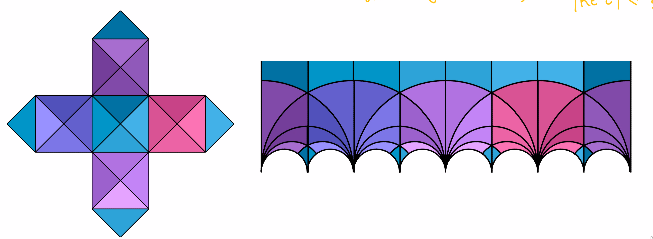
\includegraphics[width=0.8\linewidth]{squarefd} \caption{Fundamental domain
    subdivided}% \label{fig:squarefd} \end{figure} The dodecahedron and
    icosahedron correspond to the following: \begin{figure}[H] \centering
        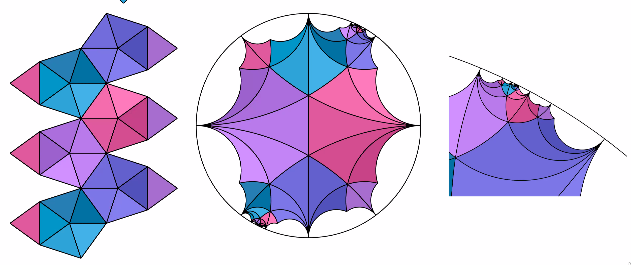
\includegraphics[width=0.8\linewidth]{icosafd} \caption{Fundamental
        domain for icosahedron}% \label{fig:icosafd} \end{figure} The cusps
        correspond to points of $5$-fold symmetry, and correspond to $0, 1, 2,
        \infty, \varphi, 1/\varphi, \ldots$, and the points converging to
        $1/\varphi$ are given by ratios $F_n/F_{n-1}$ of Fibonacci numbers.

\begin{rmk} Instead of just considering the icosahedron, we should consider an
infinite strip with the given pattern in the picture.  \end{rmk}

\section{Jordan Decomposition}% \label{sec:jordan_decomposition}

Let $\k = \ol{\k}$. Then for all $g \in G = GL(V)$, we can decompose $g$ into
Jordan blocks. In particular, we can write $g = g_s g_n$, where $g_s$ is
semisimple and $g_n$ is strictly upper triangular (in some basis). The
analogous decomposition for $\xi \in \mf{g}$ is $\xi = \xi_s + \xi_n$. Now if
$V \subseteq \k^n$ is invariant under $g$, it is invariant under both $g_s,
g_n$.

Consider the regular representation $\rho$ of $G = GL(n, \k)$ on $\k[G]$.

\begin{lem} For any $g \in G$, we have ${\rho(g)}_s = \rho(g_s)$.  \end{lem}

\begin{cor} If $G$ is an algebraic group, then $g_s, g_n \in G$ for all $g \in
G$. Moreover, if $\varphi \colon G_1 \to G_2$ is a homomorphism, then ${
\varphi(g) }_s = \varphi(g_s)$ and ${\varphi(g)}_n = \varphi(g_n)$.  \end{cor}

\begin{proof} By Chevalley, $G$ is the stabilizer of a subspace on $\k[GL(n)]$
    and therefore because $g$ stabilizes the subspace, so do $g_s, g_n$.

    For the second part, we can pull back $\varphi^* \colon \k[G_2] \to
\k[G_1]$ and then the desired result is obvious.  \end{proof}

\section{More Solvable Lie Algebras}% \label{sec:more_solvable_lie_algebras}

We will return to solvable Lie algebras. Assume $\chr \k = 0$.

\begin{thm} Let $\mf{g} \subset \mf{gl}(V)$ be a Lie subalgebra. Then $\mf{g}$
is solvable if and only if $\trace x[y,z] = 0$ for all $x,y,z \in \mf{g}$.
\end{thm}

\begin{proof} One direction is clear by Borel. Here, $\mf{g} \subset \mf{b}$ is
    contained in the subalgebra of upper-triangular matrices. In the other
    direction, the form $\trace x[y,z] \in { ( \Omega^3 \mf{g} ) }^{\mf{g}}$.
    In particular, we see that if $\mf{g} = \Lie(G)$, then this becomes a
    bi-invariant $3$-form on $G$. This gives a class in ${H^3_{\mr{dR}}(G)}^{G
    \times G}$. Now we have an exact sequence \[ 1 \to \text{unipotent radical}
    \to G \to G_{\text{reductive}} \to 1, \] and here the unipotent radical is
    homeomorphic to $\R^n$, while $G_{\text{reductive}}$ is a product of simple
    nonabelian $G_i$ and a torus up to a finite cover. Then $\operatorname{rk}
    \pi_3$ is the number of simple nonabelians, and so the morphisms $SU(2)
    \simeq S^3 \hookrightarrow {(G_i)}_{\text{compact}}$ generate $\pi_3
    \otimes \Q$.

    Now suppose that $\trace x[y,z] = 0$. Now we will show that $\mf{g}$ is
    solvable. It suffices to show that $\mf{g}' = [\mf{g}, \mf{g}]$ is
    nilpotent. By Engel, it suffices to show that any $x \in \mf{g}'$ is
    nilpotent. Consider the subalgebra \[ \mf{gl}(V) \supset \wtl{\mf{g}} =
    \qty{ \xi \mid [\xi, \mf{g}] \subset [\mf{g}, \mf{g}] } \supset \mf{g}. \]
    This is the Lie algebra of an algebraic group \[ \wtl{G} = \qty{h \mid \Ad
    (h) (\mf{g}) = \mf{g}, \Ad (h) \equiv 1 \mod [\mf{g}, \mf{g}]}. \] But then
    $\tr x \xi = 0$ for all $x \in \mf{g}', \xi \in \wtl{\mf{g}}$. Now if $x =
    \sum [y_i, z_i]$, then we have \[ \tr x \xi = \sum \tr y_i [z_i, \xi] = 0,
    \] so if $x \in \mf{g} \subset \wtl{\mf{g}}$, then $x_s \in \wtl{\mf{g}}$.
    Now considering $f(x_s) \in \wtl{\mf{g}}$, we will obtain some condition on
    $\ad f(x_s)$. These will have the same eigenvectors as $\ad x_s$. If
    $E_{ij}$ is an eigenvector of $\ad x_s$ with eigenvalue $\lambda_i -
    \lambda_j$, then it has eigenvalue $f(\lambda_i) - f(\lambda_j)$ under $\ad
    f(x_s)$. If there exists $\psi$ such that $f(\lambda_i) - f(\lambda_j)$,
    then $\ad f(x_s) = \psi(\ad x_s)$ and thus $f(x_s) \in \wtl{\mf{g}}$.

    Now if $f$ is linear over $\Q$, then $f(x_s) \in \wtl{\mf{g}}$ and $\ad
f(x_s) = f(\ad x_s)$. Next we see that $\tr x_s f(x_s) = 0$ because we can
embed $\qty{\lambda_i} \subset \C$ and then take $f(\lambda_i) =
\ol{\lambda}_i$. Then we see that $\tr x_s f(x_s) = \sum \abs{\lambda_i}^2 =
0$, and then we see that all $\lambda_i = 0$. Alternatively, if $\dim_{\Q}
\bigoplus \Q \lambda_i > 0$, then there exists a nonzero $f \colon \bigoplus \Q
\lambda_i \to \Q$, but then $f \qty(\sum \lambda_i f(\lambda_i)) = \sum
{f_i(\lambda)}^2$.  \end{proof}

\begin{defn} Define the \textit{Killing form} by \[ (x,y) \coloneqq \tr \ad(x)
\ad(y). \] \end{defn}

\begin{rmk} Killing apparently lived a very sad life and did not get the
recognition he deserved. Unfortunately, Andrei (and I) do not know more about
him.  \end{rmk}

\begin{thm} A Lie algebra $\mf{g}$ is solvable if and only if $(x, [y,z]) = 0$.
\end{thm}

\begin{proof} Consider the exact sequence \[ 0 \to Z(\mf{g}) \to \mf{g} \to \ad
\mf{g} \to 0. \] Then solvability of $\mf{g}$ is equivalent to solvability of
$\ad \mf{g}$.  \end{proof}

\begin{thm}[Cartan Criterion] A Lie algebra $\mf{g}$ is semisimple if and only
if the Killing form is nondegenerate.  \end{thm}

\begin{proof} Suppose $(-,-)$ is degenerate. Then $\mf{g}^{\perp}$ is a
    solvable ideal in $\mf{g}$. But then if $\mc{I}$ is a solvable ideal with
    $\mc{I}^{n+1} = 0$, then $\mf{a} = \mc{I}^n$ is an abelian ideal.
    Therefore, for all $x,y$, we see that \[ [\mf{a}, [y,[\mf{a}, x]]] = 0, \]
    and therefore for all $a \in \mf{a}, y \in \mf{g}$, we have $\ad (a) \ad(y)
    \ad(a) = 0$, so ${(\ad(a) \ad(y))}^2 = 0$, and thus $\tr \ad(a) \ad(y) =
    0$. But then $a \in \mf{g}^{\perp}$.  \end{proof}

\begin{cor} If $\mf{g}$ is semisimple, then $\mf{g} = \bigoplus \mf{g}_i$ is a
sum of simple nonabelians.  \end{cor}

\begin{proof} Suppose $\mf{h} \subset \mf{g}$ is an ideal. Then $\mf{h} \cap
\mf{h}^{\perp} = 0$ (because it is a solvable ideal). Note that if $\mf{h}
\subset \mf{g}$ is an ideal, then ${(h_1, h_2)}_{\mf{h}} = {(h_1,
h_2)}_{\mf{g}}$.  \end{proof}

\chapter{Geometric and topological aspects}% \label{cha:cohomology}

\section{Lie algebra cohomology}% \label{sec:semisimple_lie_algebras}

There are three kinds of properties: \begin{itemize} \item General abstract
    properties; \item Properties derived from the structure theory $\mf{g} =
    \mf{h} \oplus \bigoplus_{\alpha} \mf{g}_{\alpha}$; \item Properties derived
    from the calssification of root systems.  \end{itemize}

We will begin with the first. If $\mf{g}$ is semisimple, then:
\begin{enumerate} \item The category $\Mod_{\mr{fd}} \mf{g}$ is semisimple. In
    particular, every finite-dimension $\mf{g}$-module has the form $M =
    \bigoplus M_i$, where the $M_i$ are simple.  \item The algebra $\mf{g}$ has
    no \textit{deformations}.  \item All derivations of $\mf{g}$ are inner
    derivations. In particular, we see that $\mf{g} = \Lie(\Aut(\mf{g}))$. In
    addition, in the exact sequence \[ 0 \to Z(\mf{g}) \to \mf{g}
        \xrightarrow{\ad} \operatorname{Der} \mf{g} \to \operatorname{Out}
        \mf{g} \to 0, \] the two outside terms vanish.  \item For any Lie
        algebra $\mf{g}_{\mr{any}}$, we have \[ 0 \to \text{radical} \to
        \mf{g}_{\mf{any}} \to \mf{g}_{\mr{ss}} \to 0, \] and this exact
sequence splits into $\mf{g}_{\mr{any}} = \mf{g}_{\mr{ss}} \ltimes
\text{radical}$.  \end{enumerate} All of these pheonomena fit under the
umbrella of the vanishing of some cohomology groups.

\begin{defn} Let $\mf{g}$ be a Lie algebra over a field $\k$ and $M$ be a
    $\mf{g}$-module. We may consider the complex \[ \Hom_{\k}
        \qty({\bigwedge}^n \mf{g}, M) \ni \omega(\xi_1, \ldots, \xi_n) \qquad
        \xi_i \in \mf{g}. \] and define \[ \dd{\omega}(\xi_1, \ldots,
    \xi_{n+1}) = \sum_i {(-1)}^{i-1} \xi_i \omega (\ldots, \wh{\xi}_i, \ldots)
+ \sum_{i < j} {(-1)}^{i+j} \omega ([\xi_i, \xi_j], \ldots, \wh{\xi}_i, \ldots,
\wh{\xi}_j, \ldots). \] In the homework, we will show that $\dd^2 = 0$, so we
may define the \textit{Lie algebra cohomology} $H^n(\mf{g}, M)$.  \end{defn}

For an example in low dimension, we see that $C_0 = M \to C_1$ is given by
$\dd{\omega} (\xi_1) = \xi_1 (\omega)$, so $H^0(M) = M^{\mf{g}}$. For a more
modern definition, we see that $H^i(\mf{g}, M)$ are the derived functors of $M
\to M^{\mf{g}}$.

We may motivate this formula in the following way from the de Rham
differential. Suppose $G$ acts on a manifold $X$. This gives a morphism $\mf{g}
\to \Gamma(X, TX)$ into the vector fields. Then if $\xi_1, \ldots, \xi_{n+1}$
are vector fields on $X$ and $\omega$ is an $n$-form on $X$, we have
\begin{prop} The formula for $\dd{\omega} (\xi_1, \ldots, \xi_n)$ is the same
formula as in Lie algebra cohomology, where $\xi_i \omega$ is the Lie
derivative of $\omega$ along $\xi_i$.  \end{prop}

\begin{proof} Andrei's proof is way too confusing. This is also Proposition
12.19 in Lee's smooth manifolds book. The proof there is the same, but is done
in a much easier-to-digest way.  \end{proof}

\begin{thm} Let $\mf{g}$ be a semisimple Lie algebra over a field of
    characteristic $0$.  \begin{enumerate} \item If $M$ is irreducible and
        nontrivial, then $H^{\bullet}(\mf{g}, M) = 0$.  \item
        $H^{\bullet}(\mf{g}, \k)$ is the free anticommutative algebra on
        finitely many generators of degree contained in $\qty{3, 5, 7,
        \ldots}$. When $\k = \C$, this is the same as $H^{\bullet}(G, \C)$.
        This is also the same as the cohomology of the maximal compact
        subgroup. For example, \[ H^{\bullet}(SL(n, \C), \C) =
        H^{\bullet}(SU(n), \C) = \C\ev{\omega_3, \omega_5, \ldots,
    \omega_{2n-1}}. \] In particular, if $\mf{g}$ is semisimple, then $H^{1},
    H^2$ vanish for all $M$. Also, we have an isomorphism $H^3(\mf{g}, \k)
    \cong k^{\#\ \text{simple factors}}$, and this is just the space of
    invariant bilinar forms.  \end{enumerate} \end{thm}

\begin{proof}\leavevmode \begin{enumerate} \item Suppose $M$ is nontrivial and
    irreducible. Without loss of generality, assume $\mf{g}$ is simple and
    consider $\mf{g} \subseteq \mf{gl}(M)$. We will show that multiplication by
    $\dim \mf{g}$ is homotopic to $0$. Consider the form $B(x, y) = \tr_M xy$,
    which is nondegenerate. Then if $\qty{e_1, \ldots, e_d}, \qty{f_1, \ldots,
    f_d}$ are dual bases of $\mf{g}$, the \textit{Casimir element} $\sum e_i
    f_i$ commutes with $\mf{g}$ and is nonzero because $\tr \sum e_i f_i = \sum
    \tr e_i f_i = \dim \mf{g}$. Now we will define our homotopy by \[ h \omega
        (\xi_1, \ldots, \xi_{n-1}) = \sum e_i \omega (f_i, \xi_1, \ldots,
        \xi_{n-1}). \] Now, we compute $\dd \circ h + h \circ \dd$. We have
        \begin{align*} \dd h \omega (\xi_1, \ldots, \xi_n) &= \sum_i
            {(-1)}^{i-1} \xi_i e_* \omega (f_*, \ldots, \wh{\xi}_i, \ldots) +
            \sum_{i < j} {(-1)}^{i+j} {(-1)}^{i+j} e_* \omega (f_*, [\xi_i,
            \xi_j], \ldots) \\ \end{align*} Then writing \begin{align*}
            \dd_{\omega} (\xi_0, \xi_1, \ldots, \xi_n) ={} &\xi_0 \omega
            (\xi_1, \ldots, \xi_n) + \sum {(-1)}^i \xi_i \omega (\xi_0, \ldots,
            \wh{\xi}_i, \ldots, \xi_n)  \\ &+ \sum_i {(-1)}^i \omega ([\xi_0,
            \xi_i], \ldots) + \sum_{0 < i < j} {(-1)}^{i+j} \omega ([\xi_i,
            \xi_j], \ldots), \end{align*} we have \begin{align*} h
            \dd{\omega}(\xi_1, \ldots, \xi_n) ={} &e_* f_* \omega (\xi_1,
            \ldots, \xi_n) + \sum {(-1)}^i e_* \xi_i \omega (f_*, \ldots) \\ &+
            \sum_i {(-1)}^i e_* \omega ([f_*, \xi_i], \ldots) + \sum_{i < j}
            {(-1)}^{i+j} e_* \omega ([\xi_i, \xi_j], f_*, \ldots).
            \end{align*} Now we may verify that all of the relevant terms
            cancel, so \[ (hd + dh) \omega = e_* f_* \omega + \sum_i {(-1)}^i (
            [e_*, \xi_i] \omega (f_*, \ldots) + e_* \omega ([f_*, \xi_i],
        \ldots) ). \] The second term is given by inserting the tensor $[e_*
        \otimes f_*, \xi_i \otimes 1 + 1 \otimes \xi]$. But then $e_* \otimes
        f_*$ is an invariant tensor, so $\ad (\xi) e_* \otimes f_* = [\xi
        \otimes 1 + 1 \otimes \xi, e_* \otimes f_*] = 0$.  \item We may assume
        that $\k = \R$ or $\k = \C$, so let $G$ be a connected compact Lie
        group. We will see that $H^{\bullet}(\mf{g}) = {(\bigwedge^{\bullet}
        \mf{g})}^G \simeq H^{\bullet}(G)$. We will compute ordinary cohomology
        using the de Rham complex. First, we will note that $g \in G$ acts
        trivially on $H^{\bullet}(G)$. To see this, observe that $\xi \in
        \mf{g}$ acts on forms by the Lie derivative $L_{\xi}$, and $[L_{\xi}
        \omega] = 0$ if $\dd{\omega} = 0$ by the Cartan formula.

            Now for any compact group $G$ acting on a manifold $X$, the
            inclusion ${(\Omega^i X)}^G \to \Omega^i X$ induces an isomorphism
            on cohomology. To see this, we simply note that $\int g^* \omega
            \dd{g}$ is cohomologous to $\omega$. Therefore, we may consider
            right-invariant forms in $\Omega^i G$. But then \[ {(\Omega^i
            G)}_{\text{right invariant}} \simeq {\bigwedge}^i \mf{g}^* \simeq
        {\bigwedge}^i \mf{g}, \] and the differential on $\bigwedge^i \mf{g}^*$
        is the differential from Lie algebra cohomology. Now if we consider
        ${(\Omega^i)}^{G \times G} \simeq {(\bigwedge^i \mf{g}^*)}^G$, the
        differential vanishes. To see this, the map $g \mapsto g^{-1}$
        perserves the biinvariants but acts by ${(-1)}^i$ on $\bigwedge^i
        \mf{g}^*$, and so $\dd \mapsto -\dd$, so $\dd = 0$. Because $\mf{g}$
        acts trivially on cohomology, it is also possible to see that \[ \qty(
    {\qty({\bigwedge}^{\bullet} \mf{g}^*)}^{\mf{g}}, 0 ) \hookrightarrow \qty (
    {\bigwedge}^{\bullet} \mf{g}^*, \dd ) \] is a quasi-isomorphism. \qedhere
    \end{enumerate} \end{proof}

\begin{exm} \begin{enumerate} \item Let $\mf{g}$ be abelian. Then \[
H^{\bullet}(\mf{g}, \R) = {\bigwedge}^{\bullet} \mf{g}^* =
H^{\bullet}(\mf{g}/\Lambda, \R) = {\bigwedge}^{\bullet} H^1\qty(\prod S^1, \R).
\] \item The condition that $G$ is compact is important. Note that \[
H^{\bullet}(SL(2, \R), \R) = H^{\bullet}(S^1) \neq H^{\bullet}(S^3) =
H^{\bullet}(SU(2)) = H^{\bullet}(\mf{su}(2), \R). \] \end{enumerate} \end{exm}

Next, we will actually prove that $H^{\bullet}(\mf{g}, \k) = \k
\ev{\omega_{2d_i - 1}}_{i = 1, \ldots, \rank \mf{g}}$. In particular, by a
theorem of Hopf, this is a Hopf algebra. Similarly, if $G$ is a compact Lie
group then $H^{\bullet}(G, \R)$ is a Hopf algebra. Here are some properties of
the cohomology: \begin{itemize} \item It is graded and supercommutative.  \item
    Under the map $G \to G \times G \xrightarrow{\mu} G$ given by $g \mapsto
    (g, 1) \to g$, if we write \[ \Delta \omega = \sum \omega_i' \otimes
    \omega_i'', \] then $(1 \otimes \eta) \Delta \omega = \omega$ because
    $\Delta \omega = \omega \otimes 1 + 1 \otimes \omega + H^{>0} \otimes
    H^{>0}$.  \end{itemize}

\begin{thm}[Hopf] Any finitely generated graded supercommutative Hopf algebra
and the second property has the form $\k \ev{\omega_{m_i}}$.  \end{thm}

\begin{cor} If, additionally, our Hopf algebra is assumed to be
finite-dimensional, then all of the $m_i$ are odd.  \end{cor}

\begin{proof} Let $\omega_{m_i}$ be generators with $m_1 \leq m_2 \leq \cdots$.
    Then let $\mathcal{H}_k$ be the algebra generated by $\omega_{m_1}, \ldots,
    \omega_{m_k}$. Then we know that $\Delta \omega_{m_k} = \omega_{m_k}
    \otimes 1 + 1 \otimes \omega_{m_k} + \cdots$, so each $\mathcal{H}_k$ is a
    sub-bialgebra. Now it suffices to show that $\mathcal{H}_k =
    \mathcal{H}_{k-1} \ev{\omega_{m_k}}$.

    Suppose there is a relation $R = \sum_{i=0}^d c_i x^i = 0$ of degree $d$.
    But now if we consider the ideal $\Delta R$ modulo $1 \otimes
    \ev{\mathcal{H}_{k-1}, x^2}$, which does not contain $x$ for grading
    reasons, then we have \begin{align*} \Delta c_i &= c_i \otimes 1 + \cdots
        \\ \Delta x &= x \otimes 1 + 1 \otimes x + \cdots \\ \Delta x^n &=
        {(\Delta x)}^n = x^n \otimes 1 + nx^{n-1} \otimes x + \cdots \\ \Delta
        R &= R \otimes 1 + \pdv{x} R \otimes x + \cdots, \end{align*} and this
    must be a relation of smaller degree. Therefore we have no relations beyond
supercommutativity.  \end{proof}

Now an interesting problem is to compute the degrees of the generators. For
example, we have \[ H^{\bullet}(SU(n)) = \R \ev{\omega_3, \omega_5, \ldots,
\omega_{2n-1}}. \]

\begin{thm}[Cartier-Kostant-Gabriel-\ldots] If $\mathcal{H}$ is a
    supercommutative Hopf algebra over a field $\k$ of characteristic $0$, then
    \[ \mathcal{H} = \k G \ltimes \mathcal{U}(\mf{g}). \] where $G$ is a
    (typically finite) group and $\mf{g}$ is a Lie superalgebra over $\k$.
\end{thm}

The elements with $\Delta g = g \otimes g$ are called \textit{grouplike}, and
the elements with $\Delta \xi = \xi \otimes 1 \pm 1 \otimes \xi$ are called
\textit{primitive}. The grouplike elements give us $G$, and the primitive
elements give us $\mf{g}$. 

Now we may take the dual Hopf algebra, and this gives us another graded
supercommutative Hopf algebra. These give us algebraic supergroups over $\k$.
But this algebraic supergroup must be an odd vector space. Another consequence
of the theorem is that a commutative Hopf algebra over $\k$ has no nilpotent
elements. This implies that all group schemes over $\k$ are reduced and
therefore smooth.

Recall that if $G$ is a compact connected Lie group, then $H^{\bullet}(G, \R) =
\R \ev{\omega_{2d_i - 1}}_{i = 1, \ldots, \rank G}$.

\begin{thm} We have $\dim_{\R} H^{\bullet}(G, \R) = 2^{\rank G}$, where $\rank
G$ is the dimension of the maximal torus.  \end{thm}

We would also like to compute the $d_i$. In fact, $d_i$ are the degrees of the
generators of ${ ( S^{\bullet} \mf{g}^* ) }^G$. We know that every element of
$\mf{g}$ is conjugate to an element of $\mf{t} = \Lie T$. The normalizer of
this is the Weyl group $W$. Now, by definition, we have \[ {(S^{\bullet}
\mf{t}^*)}^W = \R[\mf{t}/W], \] and this is free on some generators $p_{d_i}$
of degree $\abs{p_{d_i}} = d_i$ for $i = 1, \ldots, \dim \mf{t} = \rk G$.

\begin{thm} The $d_i$ defined in the various ways are the same numbers and are
called \textit{exponents} of $G$.  \end{thm}

\begin{exm} For $G = U(n)$, we have $\qty{d_i} = \qty{1, 2, \ldots, n}$ and
    $p_d = \tr \xi^d$. Alternatively, we can use the coefficients of the
    characteristic polynomial. In addition, we see that \[ H^{\bullet}(U(n)) =
    \R \ev{\omega_1, \omega_3, \omega_5, \ldots, \omega_{2n-1}}, \] and
    ${\qty(\bigwedge^{\bullet} \mf{g}^*)}^G$ is generated by $\omega_1(\xi) =
    \tr \xi, \omega_3 (\xi_1, \xi_2, \xi_3) = \tr \xi_1 [\xi_2, \xi_3]$, and in
    general \[ \omega_d(\xi_1, \ldots, \xi_d) = \sum_{\sigma \in S(d) /
    (123\ldots d)} {(-1)}^{\sigma} \tr \prod_{i=1}^d \xi_{\sigma(i)}. \] In
this formula, we observe that $d$ must be odd.  \end{exm}

\begin{proof}[Proof of Theorem 3.2.8] Use the Molien series. We have \[ \dim
V^G = \int_G \tr_V g \dd{g} = \frac{1}{\abs{W}} \int_T \tr_V g \cdot
\det_{\mf{g}/\mf{t}} (1 - \Ad(t)) \dd_{\mr{Haar}} t. \] Setting $V =
\bigwedge^{\bullet} \mf{g}$, we see that \[ \tr_V g = \det_{\mf{g}} (1 +
    \Ad(g)) = 2^{\rank} \det_{\mf{g}/\mf{t}} (1 + \Ad(t)). \] This now gives us
    \[ 2^{\rank} \frac{1}{W} \int_T \det_{\mf{g}/\mf{t}} (1 - \Ad(t^2))
    \dd_{\mr{Haar}} t = 2^{\rank} \] by change of variables.  \end{proof}

\section{Classifying Spaces and Flag Varieties}%
\label{sec:classifying_spaces_and_flag_varieties}

We already know that $H^{\bullet}(G) = \R \ev{\omega_{2d_i - 1}}$. On the other
hand, we know the cohomology of the flag manifold $H^{\bullet}(G/T)$ is all
even, and finally we have the cohomology \[ H^{\bullet}(BG) =
H^{\bullet}(\mr{pt} /G) = {(S^{2\bullet} \mf{g}^*)}^G = {(S^{\bullet}
\mf{t}^*)}^W. \] On the other hand, we have \[ H^{2\bullet}(G/T) =
{(S^{\bullet} \mf{t}^*)} / {(S^{\bullet} \mf{t}^*)}^W_{>0}. \] For $G = U(n)$,
this becomes the space of polynomials divided by symmetric polynomials of
positive degree and has dimension $n! = \abs{W}$. This is the fiber over $0$ of
the map $\mf{t} \to \mf{t} / W$. To define $BG$, consider the category of
spaces with a free action of $G$ (equivalently principal $G$-bundles) for any
group $G$. Given a commutative diagram \begin{equation*} \begin{tikzcd} G
\ar[hookrightarrow]{r} \ar{d}{\varphi_G} & X \ar{d}{\varphi_X} \\ G'
\ar[hookrightarrow]{r} & X' \end{tikzcd} \end{equation*} with $\varphi(g \cdot
x) = \varphi(g) \cdot \varphi(x)$, we would like to consider the possibilities
for $\varphi_X$ for a fixed $\varphi_G$. If we consider the graph of
$\varphi_X$, this is just a section of $X \times X' / X$ because $G$ acts
freely, this is the same as a section of $(X \times X')/G \to X/G$.

\begin{thm} If $X'$ is contractible, then there exists a unique $\varphi_X
\colon X \to X'$ compatible with $\varphi_G$.  \end{thm}

\begin{prop} For any compact group $G$, there exists a contractible space $EG$
with a free $G$-action.  \end{prop}

\begin{cor}\leavevmode \begin{enumerate} \item $EG$ is unique up to homotopy.
    \item $EG$ is functorial in $G$.  \item For any free action of $G$ on $X$,
        the map $X \to X/G$ is the pullback of \begin{equation*} \begin{tikzcd}
            X \ar{r} \ar{d} & EG \ar{d} \\ X/G \ar{r} & BG \end{tikzcd}
        \end{equation*} for some map $X/G \to BG$. Therefore, we see that \[
\qty{\text{principal $G$-bundles over $B$}} = [B, BG]. \] \end{enumerate}
\end{cor}

\begin{proof}[Proof of proposition] For all $G$ compact, there exists an
    embedding $G \subseteq U(n)$, so it suffices to consider $U(n)$. Consider
    the embedding $U(n) \hookrightarrow { \mr{Mat}(n, N) }_{\rank = n}$ for
    some $N \gg 0$. For example, we have the action of $U(1)$ on $\C^n
    \setminus 0 \simeq S^{N-1}$, so we can consider $S^{\infty}$, which is
    contractible. Therefore we have $BU(1) = S^{\infty} / U(1) =
    \C\P^{\infty}$.

    In general, we can consider the action of $U(n)$ on \[ \mr{Mat}(n, N)
    \setminus \qty{\rank < n} \supseteq \qty{X \mid XX^* = 1_n}, \] and this
    last space becomes contractible as $N \to \infty$. To see this, it sits
    inside of ${(S^N)}^n$, and thus as $N \to \infty$, we obtain a contractible
    subspace of ${(S^{\infty})}^n$. Finally, we have $BU(n) = \mr{Gr}(n,
    \infty)$.  \end{proof}

Therefore, we have a tautological $U(n)$-bundle on $\mr{Gr}(n, \infty)$ and a
tautological $\C^n$-bundle where the fiber above a subspace is the subspace
itself. The vector bundle is the associated bundle of the $U(n)$-bundle and the
$U(n)$-bundle is the bundle of unitary operators on the vector bundle. Also, we
have proved that \[ \qty{\text{complex vector bundles of rank $n$ over $B$}}
\longleftrightarrow [B, \mr{Gr}(n, \infty)]. \] The same statement holds for
$O(n)$, real vector bundles, and the real Grassmannian. Explicitly over $B$,
consider the exact sequence \[ 0 \to \ker \to \C^N_B \to V \to 0. \] Now the
kernel defines a map $B \to \mr{Gr}(N - n, N) \simeq \mr{Gr}(n, N)$. Taking $N
\to \infty$, we obtain the desired result.

\begin{rmk} The spaces $EG$ and $BG$ are naturally approximated by algebraic
varieties such as $\mr{Gr}(n, N)$ and are therefore ind-schemes.  \end{rmk}

We want to show that $\R^{\infty} \setminus 0$ is contractible. We can consider
the function $T$ on $\R^{\infty} \setminus 0$ given by $T(x_1, x_2, \ldots, 0,
\ldots) = (0, x_1, x_2, \ldots)$. Then $x, Tx$ are never collinear for $x \neq
0$ and thus $T$ is homotopic to the identity. But then $Tx$ is never collinear
to $e_1 = (1, 0, \ldots,)$ and therefore $T$ is nullhomotopic. We also see that
$C^{\infty} \setminus 0$ is contractible. Also, $S^{\infty} \sim \R^{\infty}
\setminus 0$ is contractible and so are Stiefel manifolds \[ \qty{v_1, \ldots,
v_n \in \C^{\infty} \mid v_i\ \text{are linearly independent}}. \] The Stiefel
manifold has a free action of $GL(n, \C)$, so this is $EGL(n, \C)$. We also see
that $BGL(n, \C) = \mr{Gr}(n, \infty, \C)$. We know that the maximal compact
subgroup of $G$ is homotopy equivalent to $G$, so $BGL(n, \C) = BU(n)$.

\begin{rmk} The high-brow way that we prove that all of these spaces are
    contractible is by proving that they are weakly contractible, and then
    smashing the remaining part that weakly contractible implies contractible
    for spaces with the homotopy type of a CW complex.  \end{rmk}

Now the cohomology $H^{\bullet}(B, G)$ is intimately connected to
characteristic classes for principal $G$-bundles. If $G$ acts on a manifold
$M$, we have a map $\mf{g} = \Lie(G) \to \mr{Vect}(M)$, so we may consider the
Lie derivative $L_x \colon \Omega^k M \to \Omega^k M$ for $x \in \mf{g}$. For
the Lie derivatives, recall the identity $[L_x, \iota_y] = \iota_{[x,y]}$. This
gives us a super Lie algebra $\wh{\mf{g}}$ with $\wh{\mf{g}}_1 = \C_{\dd}$,
$\wh{\mf{g}}_0 = \mf{g}$, and $\wh{\mf{g}}_{-1} \cong \Ad \mf{g}$. This gives
us the super-Lie bracket \[ [a,b] = ab - {(-1)}^{\abs{a} \abs{b}} ba. \] Now we
see that $[\wh{\mf{g}}_1, \wh{\mf{g}}_0] = 0$, $[\wh{\mf{g}}_1,
\wh{\mf{g}}_{-1}]$ is given by the Cartan formula, and $[\wh{\mf{g}}_0,
\wh{\mf{g}}_{-1}]$ is the adjoint action of $\mf{g}$ on itself. Therefore, if
$M$ is a manifold with a $G$-action, then $\Omega^{\bullet} M$ is a
supercommutative DG algebra with an action of $\wh{\mf{g}}$.

If the action of $G$ is free, we may choose a $G$-invariant metric on $M$. For
every $v \in T_m M$, we have its projection onto $T_m Gm \simeq \mf{g}$. This
gives us a connection, which is a $G$-invariant $1$-form with values in
$\mf{g}$ and thus gives us a map \[ \alpha \colon \mf{g}^* \to \Omega^1 M
\qquad [\alpha(\xi)] (\iota_x) = \ev{\xi, x}. \] Therefore, if a map
$\wh{\mf{g}} \to \mc{A}^{\bullet}$, where $\mc{A}$ is a supercommutative DG
algebra means that $G$ acts on $M$, we would like to give an interpretation of
a connection $\alpha \colon \mf{g}^* \to \mc{A}^1$ such that $[\alpha(\xi)]
(\iota_x) = \ev{\xi, x}$.

\begin{thm} There exists a unique acyclic supercommutative DG algebra with
$H^0(\mc{A}^{\bullet}) = \C, H^i(\mc{A}^{\bullet}) = 0, i > 0$. We will denote
this universal algebra by $\mathbb{E}$.  \end{thm}

\begin{proof} Set $\mc{A}^0 = \C$ and $\mc{A}^1 = \alpha(\mf{g}^*)$ with $L_x$
    acting by the coadjoint action. We set $\dd \colon \mc{A}^0 \to \mc{A}^1$
    to be the zero map. We also set $\iota_x(\alpha(\xi)) = \ev{\xi, x}$.
    Because $\dd \colon \mc{A}^1 \to \mc{A}^2$ must be an isomorphism, we see
    that $\mc{A}^2 = \beta(\mf{g}^*) \oplus \bigwedge^2 \mc{A}^1$ with the
    coadjoint action of $\mf{g}$. Then we define $i_x$ by \[ i_x
    \dd{\alpha(\xi)} = L_x \alpha(\xi) - \dd i_x \alpha(\xi) = L_x \alpha(\xi).
\qedhere \] \end{proof}

Note that $\E$ looks like $\Omega^{\bullet} \mf{g}$, which are polynomials in
$x$ multiplied by $\bigwedge \dd{x_i}$. For $\beta \in \mc{A}^2$ and $\alpha
\in \mc{A}^1$, we can define $\dd^*{\beta}(\xi) = \alpha, \dd^* \alpha(\xi) =
0$. Therefore, $\dd^*$ is a derivation, and the Laplacian \[ [\dd^*, \dd] =
\dd^* \dd + \dd \dd^* \] is the identity on $\mc{A}^1$ and $\mc{A}^2$. This
implies that multiplication by $(k+\ell)$ on ${(\E^1)}^k {(\E^2)}^{\ell}$ is
homotopic to the identity and thus $H^{\bullet}(\E) = \C$.

Now we return to our manifold $M$ and base $B = M/G$. Then the image of
$H^{\bullet}(B) \hookrightarrow H^{\bullet}(M)$ are the so-called \textit{basic
forms}, which vanish on $\iota_x$ (horizontal) and are $G$-invariant. In
particular, they are killed by both $\iota_x, L_x$. Then the map
$H^{\bullet}(M) \twoheadrightarrow H^{\bullet}(G)$ has kernel the horizontal
forms, so we need to consider the horizontal forms.

\begin{prop} Horizontal forms are generated by \textit{curvatures}, which have
    the form \[ \beta(\xi) + \delta \alpha(\xi), \] where $\delta$ is the map
$\mf{g}^* \to \bigwedge^2 \E^1$ given by the transpose of the Lie bracket.
\end{prop}

We now have \[ \iota_x (\beta(\xi) + \delta \alpha(\xi)) = \alpha(\ad_x^* \xi)
    + \alpha(\xi) [x,-] = 0 \] because $\alpha(\xi)[x,-] = -\alpha(\ad_x \xi)$.
    Therefore we can write \[ \E = {\bigwedge}^{\bullet} \alpha(\xi) \otimes
    S^{\bullet}(\text{curvatures}) = {\bigwedge}^{\bullet} \alpha(\xi) \otimes
S^{\bullet} \beta(\xi). \] Therefore, we have $\E_{\text{horizontal}} =
S^{\bullet} \mf{g}^*$ and $\E_{\text{basic}} = {(S^{\bullet} \mf{g}^*)}^G$ with
zero differential, so we have $H^{2 \bullet}(\E_{\text{basic}}) = {(S^{\bullet}
\mf{g}^*)}^G$. Now we have a \textit{transgression}\footnote{This is the same
as the transgression map in the Serre spectral sequence.} map $H^{2
m}(\E_{\text{basic}}) \to H^{2 m-1}(G)$, which is the ``inverse'' $\pi \circ
\frac{\dd^*}{m} \colon \E^G \to { \qty( \bigwedge^{\bullet} \mf{g}^* ) }^G$ of
the differential. This vanishes on ${ \qty( { ( S^{\bullet} \mf{g} ) }^2_{>0} )
}^2$.

\begin{cor} $\E_{\text{horizontal}} = S^{\bullet}(\text{curvatures})$. This is
because $\iota_{\xi} \colon \mf{g} \otimes \mf{g}^* \to \C$ is a perfect
pairing.  \end{cor}

In some sense, we have proven that \begin{thm} $H^{\bullet(BG, \C)} \simeq
{(S^{\bullet} \mf{g}^*)}^G$.  \end{thm}

However, we would like to discuss $H^{\bullet}(G)$. Now we want to describe the
transgression. If $p \in H^{\bullet}(BG)$, then want to compute $\dd^{-1}(p)
\in H^{\bullet - 1}(EG)$, and then we can restrict this to $H^{\bullet}(G)$ by
killing the horizontal forms. Therefore, polynomial functions on $\mf{g}$ map
to polynomial differential forms on $\mf{g}$ by $\dd^*$. This gives us
something like \[ p(x) \mapsto \sum_{\partial_i} p(x) \otimes \xi^i \mapsto
\text{substitute $x = -[\xi, \xi]$} \] and this takes polynomials of degree $m$
to elements of degree $2m-1$. Now in the chain \[ \qty( {(S^m\mf{g}^*)}^G, 0 )
\to \cdots \to \qty(\qty({\bigwedge}^{2m-1} \mf{g}^*), 0), \] the choice of
$\dd^{-1}$ does not matter. Also, this map is zero on ${\qty({(S^{>0}
\mf{g}^*)}^G)}^2$ because $\dd^{-1} (p_1p_2) = p_1 \dd^{-1}p_2$ if $\deg p_1,
\deg p_2 > 0$, which is killed by transgression. Therefore, primitive elements
of ${(S^{\bullet}\mf{g}^*)}^G$ map isomorphically onto primitive elements of
${\qty(\bigwedge^{\bullet} \mf{g}^*)}^G$. Now we have explained the
relationship between $H^{\bullet}(G)$ and $H^{\bullet}(BG)$. 

We now want to add the third vertex of the triangle, which is
$H^{\bullet}(G/T)$. Recall that any element of $\mf{g}$ is conjugate to some
element of $\mf{t}$ and that ${(S^{\bullet} \mf{g}^*)}^G = {(S^{\bullet}
\mf{t}^*)}^W$, which is a free algebra. Therefore, \[ H^{2\bullet}(G/T) =
S^{\bullet} \mf{t^*} / {(S^{>0} \mf{t}^*)}^W. \] We will see that this is free
over ${(S^{\bullet} \mf{t}^*)}^W$.  \begin{exm} For $G = SU(2)$ and $G/T =
    S^2$, we have $\Lie \mf{t} = \R$ and $W = \qty{\pm 1}$, and also $H^2(S^2)
    = \C[x] / (x^2)$.  \end{exm}

Now we have a map $S^{\bullet} \mf{t}^* / {(S^{>0} \mf{t}^*)}^W \to H^{2
\bullet}(G/T)$ because the image of the map $G/T \to BT \to BG$ is a point, so
we have to kill all positive degree elements in $H^{\bullet}(BG)$.

\begin{thm}[Chevalley-Sheppard-Tod] Let $\Gamma \subset GL(V)$ be finite. Then
    the following are equivalent: \begin{enumerate} \item $\Gamma$ is generated
        by complex reflections $r$ such that $\mr{rk}(r-1) = 1$.  \item $\C[V]
        = R$ is free over the invariants $S = {\C[V]}^{\Gamma}$.  \item $S =
\C[p_1, \ldots, p_{\dim V}]$.  \end{enumerate} There is a classification of all
such groups generated by complex reflections, but Andrei does not remember what
it is.  \end{thm}

The key to the proof of this theorem is \textit{divided difference operators:}
If $s_{\alpha}$ is a reflection, then $V^s$ is a hyperplane, so for all $f \in
R$, we may consider $\frac{ f - s_{\alpha} \cdot f }{\alpha}$. This vanishes on
$V^s$, lowers the degree by $1$, and commutes with $x$. For example, we could
choose \[ \frac{f(x_1, x_2, \ldots) - f(x_2, x_1, \ldots)}{x_1 - x_2}. \]

\begin{proof} Let $e_1, e_2, \ldots$ be a basis of $R/S^{>0} \cdot R$. We will
    show that it is also a basis of $R$ over $S$. Suppose there exists a
    relation $\sum g_i e_i = 0$, where $g_i \in S$. Then either $g_1 \in
    \sum_{i > 0} S g_i$ or $e_1 \in RS^{>0}$. Inducting on the degree of $e_1$,
    if $\deg e_1 = 0$, then \[ g_1 = - \sum_{i > 1} g_i e_i. \] Averaging over
    $\Gamma$, we obtain the desired expression. If $\deg e_1 > 0$, then we can
    apply divided difference operators to reduce the degree. The divided
    differences of some function $f$ all vanish only when $s_{\alpha} f = f$
    for all $\alpha$, which is equivalent to $f \in R^G = S$. Therefore we can
    assume $f \in S^{>0}$, so if $g_1 = \sum c_i g_i$, then \[ e_1, e_2 + c_2
        e_1, e_3 + c_3 e_1, e_4 + c_4 e_1, \ldots \] form another basis of
        $R/S^{>0}$. But now we obtain a shorter relation \[ \sum g_i e_i = g_2
        (e_2 + c_2 e_2) + g_3(e_3 + c_3 e_1) + \cdots \] Therefore we have
        proved freeness. Finally, we see that the rank of $R$ over $S$ is $\deg
        (V \to V/\Gamma) = \abs{\Gamma}$.

    Now note that $V \to V/\Gamma$ is flat. Therefore $V/\Gamma$ is smooth.
    Recall that if $X$ is a scheme, a point $p \in X$ is smooth if and only if
    a minimal resolution of $\cdots \to \mc{O}_X \to \mc{O}_p$ is
    finite.\footnote{You can choose your favorite singular variety and try to
    find a finite resolution}. The most important point to check is $0$. Here,
    have a finite resolution \[ \underbrace{\cdots \cdots}_{\text{finite}} \to
    S \to S/S^{>0} \to 0, \] so after tensoring with $R$, flatness gives us
    finiteness for $R \to R/RS^{>0}$.

    To prove the final leg, we will use Molien series. Recall that $V/{\Gamma}$
    is a cone with vertex $0$ and is also smooth, so it must be affine space.
    Recall that $S = \bigoplus_{i \geq 0} S_i$, where $S_0 = \C$. Then
    \begin{align*} \frac{1}{\prod(1-t^{m_i})} &= \sum_i t^i S_i \\ &=
        \frac{1}{\abs{\Gamma}} \sum_{\gamma \in \Gamma} \det \frac{1}{1- t
        \gamma} \\ &= \frac{1}{\Gamma} \qty(\frac{1}{1-t} \dim V +
        \sum_{\text{reflections}} \frac{1}{{(1-t)}^{\dim V - 1}} \cdots +
        O\qty(\frac{1}{{(1-t)}^{\dim V - 2}})).  \end{align*} This implies that
        the number of generators is $\dim V/\Gamma = \dim V$. This implies that
        $\abs{\Gamma} = \prod m_i$. For example, if $G = SU(n)$, then $\abs{W}
        = n! = n(n-1)(n-2) \cdots 2$, and the exponents are $1, \ldots, n$. The
        next term in the expansion gives us the subgroup of all reflections
        fixing $\alpha = 0$ in $\Gamma$, and in fact it is cyclic and contained
        in the roots of unity. Denote a generator by $\zeta_k$. Then we have
        \begin{align*} \frac{1}{\abs{\Gamma}} \qty( \sum_s \frac{1}{\det(1-ts)}
            + o(\cdots) ) &= \sum \frac{1}{{(1-t)}^{r-1}} \sum_{i=1}^{k-1}
            \frac{1}{1-\zeta_k^i t} \\ &= \sum \frac{1}{{(1-t)}^{r-1}}
        \frac{k-1}{2} \\ &= \frac{1}{{(1-t)}^{r-1}} \frac{\#
    \text{reflections}}{2} + o(\ldots).  \end{align*} This implies that $\#
    \text{reflections} = \sum (m_i - 1)$. For example, for $\Gamma = S_n$, we
    have $\binom{n}{2} = (1-1) + (2-1) + \cdots + (n-1)$. Now set $\Gamma'
    \subset \Gamma$ be the subgroup generated by reflections. Then $\C[p_i] = S
    \subset S' = R^{\Gamma'} = \C[p_i']$, where $p_i'$ has degree $m_i'$ and
    $p_i$ has degree $m_i$. If we order $m_1 \leq \cdots \leq m_r$ and $m_1'
    \leq \cdots \leq m_r'$, then $m_i \geq m_i'$ because otherwise the $p_1,
    \ldots, p_i$ would be algebraically dependent. Thus $\sum (m_i - 1) \geq
    \sum (m_i' - 1)$ and in in fact the inequality is strict unless $m_i =
    m_i'$ for all $i$. However, both sums count reflections, which is the same
    for $\gamma, \gamma'$, so in fact $m_i = m_i'$. This implies that $\prod
    m_i = \prod m_i'$, and thus $\abs{\Gamma} = \abs{\Gamma'}$, so $\Gamma =
    \Gamma'$.  \end{proof}

Now we have a diagram \begin{equation*} \begin{tikzcd} H^{\bullet}(G/T, \C) &
    S^{\bullet} \mf{t}^* \ar[equal]{r} \ar{l} \ar{d}{\lambda \mapsto
    \lambda([x_1, x_2])} & H^{\bullet}(BT) \\ \text{invariant differential
forms} \ar{u} & {\qty({\bigwedge}^{\bullet}{(\mf{g}/\mf{t})}^*)}^T \end{tikzcd}
\end{equation*} which commutes. In particular, $H^{\bullet}(G/T, \C)$ is the
regular representation of the Weyl group, which follows from the Lefschetz
fixed point formula, which states that if $f \colon M \to M$, then we have \[
\sum_{f(m) = m} \operatorname{mult}(m) = \sum_i {(-1)}^i \tr_{H^i(M)} f^*, \]
which says that the number of fixed points with multiplicity is equal to the
intersection product of $\Delta$ and $\Gamma(f)$. In our case, $w \neq 1$ has
no fixed points and thus its trace vanishes. For $w = 1$, all points are fixed,
so we obtain $\chi(G/T) = \abs{W}$.

Now recall that $H^{2k}(G/T) \xleftarrow{c_i} S^k \mf{t}^*$. Then $\lambda \in
\mf{t}^*$ maps to a $G$-invarint $2$-form that restricts to $\lambda([x,y])$ at
the origin and that $H^{\bullet}(G/T)$ is the regular representation of $W$.
But then we see that ${H^{\bullet}(G/T)}^W = H^0$ and thus ${(S^{>0}
\mf{t}^*)}^W \to 0$. This also follows from the fact that the composition $G/T
\to BG \to BG$ maps $G/T$ to a point. Therefore we have a map \[ S^{\bullet}
\mf{t}^* / {(S^{>0} \mf{t}^*)}^W. \] Both spaces have dimension $W$, but we
want to know if this is an isomorphism. Equivalently, we want to know whether
the cohomology of $G/T$ is generated by $c_1(\text{taut})$. Both of these are
$0$-dimensional Gorenstein rings. Of course, we have $H^{\dim M} = \C \cdot
[M]$ for any closed manifold $M$, and we call this the \textit{socle}. This has
dimension $1$ as a vector space. In addition, we have a perfect pairing \[ H^k
\otimes H^{\dim M - k} \ni \alpha \otimes \beta \mapsto \int_M \alpha \smile
\beta, \] and in particular $\dim H^k = \dim H^{\dim M - k}$. 

Another important example is a $0$-dimensional complete intersection $Z \subset
\A^d$. This has \[ \mc{O}_Z = \k[x_1, \ldots, x_d]/(f_1, \ldots, f_d), \] where
$f_1, \ldots, f_d$ is a regular sequence. For example, a dimension $0$
subscheme of the plane generated by a monomial ideal is Gorenstein if and only
if it is generated by two elements. Equivalently, its Young diagram is a
rectangle. Then the socle of $\mc{O}_Z$ is spanned by $\k \det \qty(
\pdv{f_i}{x_j} )$. In the case of a monomial ideal $(x_1^{d_1}, x_2^{d_2})$,
this is spanned by $x_1^{d_1-1} x_2^{d_2-1}$. Now a map between Gorenstein
rings is injective if and only if it preserves the socle. Then we know that
$S^{\bullet} \mf{t}^W = \C[p_1, \ldots, p_r]$, where $r$ is the rank, so $I =
(p_1, \ldots, p_r)$. Therefore $S^{\bullet} \mf{t}^* / {(S^{>0}\mf{t}^*)}^W$ is
a complete intersection. It has socle given by \[ \C \det \qty( \pdv{p_i}{x_j}
) = \C \prod \text{roots} \] and is the first anti-invariant $J$. This means
$s_{\alpha} J = -J$ and thus the socle is the sign representation of $W$. But
then any $f$ with $s_{\alpha} f = -f$ has to vanish along $\alpha = 0$, so
$\alpha \mid f$. In particular, $\prod \alpha \mid J$. We conclude that the
socle of $S^{\bullet} \mf{t}^* / {(S^{>0} \mf{t}^*)}^W$ is $\C \cdot \prod
\alpha$ with \[ (f,g) \to \frac{\text{antisymmetrize}(fg)}{\prod \alpha}. \]
Now it suffices to check where $\prod \alpha$ goes in $H^{\bullet}(G/T)$. We
know that $\prod \alpha$ is the volume form on $\mf{g}/\mf{t}$, so it goes to
${ H^{\mr{top}}(G/T) }^G$, as desired.

\begin{rmk} There are other approaches to proving this result. Let $M =
    \mr{Gr}(k, n)$ and consider the locus \[ \text{diag} = \qty{L_1, L_2
    \subset \C^n \mid \dim L_1 = k, L_1 \to \C^n \to \C^n/L_2 = 0}. \] This is
    the zero locus of a section of $\Hom(L_1, \C^n/L_2)$, where $L_1, L_2$ are
    the tautological bundles. This has rank $k(n-k)$ and thus $Gr(k, n) =
    U(n)/U(k) \times U(n-k)$. Now in $H^{\bullet}(M \times M)$, the class
    $[\text{diag}]$ is given by the characteristic classes of $L_1, L_2$. Like
    in Lefschetz, this acts by the identity operator on $H^{\bullet}(M)$ and
    thus $H^{\bullet}(M)$ is spanned by the characteristic classes of $L_1$.
\end{rmk}

It remains to discuss the relationship between $H^{\bullet}(G)$ and
$H^{\bullet}(G/T)$. In principle, we can consider $T \hookrightarrow G \to
G/T$, but studying this requires spectral sequences. Alternatively, we will
study this using the Weyl integration formula. Recall that the map \[ G/T
\times T \to G \qquad (g,t) \mapsto gtg^{-1} \] is generically
$\abs{W}$-to-$1$. Therefore we have a map \[ G/T \times T \to G/T \times_W T
\to G, \] and because the action $(g,t) \mapsto (gw^{-1}, wtw^{-1})$ is free,
the middle term is a smooth manifold. This gives us a map $H^{\bullet}(G) \to
{H(G/T \times T)}^W$. This is a map between Gorenstein rings and is injective
on the socle by inspection. Thus it remains to compute the dimension. By the
K\"unneth formula, we have \[ H^{\bullet}(G/T \times T) = H^{\bullet}(G/T)
\otimes H^{\bullet}(T). \] The first term is the regular representation of $W$
and the second term is $\bigwedge^{\bullet} \mf{t}^*$ with the natural $W$
action. But then we see that ${ H(G/T \times T) }^W$ has dimension $\dim
\bigwedge^{\bullet} \mf{t}^* = 2^r$. Chasing equivalences, we have \[
{(\Omega^{\bullet} \mf{t})}^W = {\qty({\bigwedge}^{\bullet} \mf{t}^* \otimes
S^{\bullet} \mf{t}^*)}^W = {\bigwedge}_{\k} [\dd{p_1}, \ldots, \dd{p_r}]. \]
Here, all elements of $S^{\bullet} \mf{t}^*$ have their degrees doubled. In
particular, $\deg \dd{p_i} = 2 m_i - 1$.

\begin{rmks} Recall that Lie algebra cohomology give the derived functors of $M
    \to M^{\mf{g}} = \Hom(\k, M)$. This is computed by resolving, taking
    invariants, and then taking the cohomology. This is a general principle in
    homological algebra, and in fact we can apply this to topological spaces.
    If $G$ acts freely on $M$, then $M/G$ is nice (a smooth manifold) and
    therefore is nice. Otherwise, it is better to consider $(M \times EG)/G$
    and the fibration $M \hookrightarrow (M \times EG)/G \to BG$. Then we can
    define the \textit{equivariant cohomology} \[ H^{\bullet}_G(M) =
    H^{\bullet}((M \times EG)/G), \] and this is a module over
    $H_G^{\bullet}(\mr{pt}) = H^{bullet}(BG)$. Then we can view $\Spec
    H_G^{\bullet}(M)$ (here the $\Spec$ is taken as a superscheme) as a sheaf
    over $\mf{t}^*/W$. If $G$ acts on $M$ freely, then $(M \times EG)/G$ is
    homotopy equivalent to $M/G$. The module structure over $H^{\bullet}(EG)$
    via $H^{\bullet}(BG) \to H^{\bullet}(EG) = H^0$. Now we obtain the
    skyscraper sheaf over $\mf{t}^*/W$ with stalk $H^{\bullet}(M)$ at the
    origin.

    In this language, we have $H_T^{\bullet}(G/T) = S^{\bullet} \mf{t}^*
\otimes_{{(S^{\bullet} \mf{t}^*)}^W} S^{\bullet} \mf{t}^*$, and this has a map
to $H^{\bullet}(G/T)$ killing the positive degree part of the first factor of
the tensor product. This recovers the cohomology of $H^{\bullet}(G/T)$ that we
computed before.  \end{rmks}

Now let $V$ be a rank $r$ vector bundle on $X$. Then $V$ is given by a map $X
\to BU(r) = \mr{Gr}(r, \infty)$. This induces a map $H^*(BU(r), \Z) \to H^*(X,
\Z)$. Now there is a cell decomposition $\mr{Gr}(r, N)$ into \textit{Schubert
cells}, which is given by the row reduced echelon form of a matrix in
$\mr{Gr}(r, N)$. Now this gives a basis \[ H^*(\mr{Gr}(r, N), \Z) = \bigoplus
\Z[\Sigma], \] where $\Sigma$ ranges over the Schubert cells. Then the
character \[ \sum_{\sigma \in S(r)} {(-1)}^{\sigma} x^{\sigma \cdot (\lambda +
\rho) - \rho} / \prod (x_i - x_j) \] is the character of an irreducible
representation of $U(r)$. Now in terms of the characteristic classes, pulling
back $\Z[e_1, \ldots, e_r]$ gives us classes $c_k(V) \in H^{2k}(X)$, where
$e_i$ are the elementary symmetric polynomials.

Now recall that $\mr{Gr}(N, r)$ parameterizes surjections $\C^N \to L^r$, and
if $X \xrightarrow{\varphi} [\mathfrak{S}]$, then we know $\mf{S}$ is a locus
where a section of $L$ vanishes, and $V = \varphi^* L$. Then $C_r(V) =
C_{\mr{top}}(V)$. Thus if $X$ is a complex manifold, $TX$ has rank $\dim X$, so
$c_{\mr{top}}(TX)$ is the locus where a vector field vanishes, so \[ \int_{[X]}
c_{\mr{top}}(TX) = \chi(X) \] Now $c_1$ parameterizes the locus where $r$
generic sections have rank $r-1$, or equivalently $\det V = 0$. Therefore
$c_1(V) = c_1 \qty(\bigwedge^r V)$. Then $c_k$ describes the locus where
$r-k+1$ sections have rank $r-k$. Then the splitting principle tells us that we
can write $\sum c_k(V) = \prod (1 + x_i)$, where $x_i$ are the Chern roots.
This is because if $0 \to V_1 \to V \to V_2 \to 0$ is an exact sequence, then
$c(V) = c(V_1) c(V_2)$.

Now we will consider the case of a line bundle $V = \mc{L}$. Then the curvature
of $\mc{L}$ is a class in $H^2(X, \R)$. Then we can trivialize away from the
zero locus of a section $s = 0$, If we draw a loop in the total space of
$\mc{L}$ over $X \setminus x$, then this may not be trivial. If the loop around
$D_2$ trivial, then $\int_{D_2} \mr{curv} = 0$, but if there is a zero in the
loop, then the integral is the total angle of rotation $2 \pi$ times the order
of vanishing. Thus $c_1 = \frac{\mr{curv}}{2\pi}$ and $x_1 = \frac{t_1}{2\pi}$.

Now if $\pi \colon \wh{X} \to X$ is the flag bundle of $V$, then $\pi^* V =
\mc{L}_1 \oplus \cdots \oplus \mc{L}_r$. Then \[ \pi^*(c(V)) = \prod_{i=1}^r (1
    + c_1(\mc{L}_i)). \] Now we can use this to prove that \[
\qty[\mf{S}_{\tiny\ydiagram{1,1,1,1}}] = e_k(x_1, \ldots, x_r). \]

To see this, note that every symmetric polynomial of degree $k$ is determined
uniquely by its values on $x = (x_1, \ldots, x_k, 0, \ldots, 0)$. It is enough
to consider vector bundles $V = V' \oplus \C^{r-k}$, where $V' = \mc{L}_1
\oplus \cdots \oplus \mc{L}_k$ is a sum of line bundles. Then if $s_1, \ldots,
s_k$ are sections of $\mc{L}_1, \ldots, \mc{L}_k$, then all $s_1, \ldots, s_k$
must vanish, so $e_k(x) = x_1 x_2 \cdots x_k$.

Now we want to see that $[\mf{S}_{\lambda}] = s_{\lambda}(x)$ using equivariant
cohomology. Consider the action of $GL(N)$ on $\mr{Gr}(r, N)$. It is easy to
see that the Schubert classes are preserved by the Borel subgroup. Now there is
no difference if we take the Borel or the maximal torus $A$, so we have a map
\[ \Spec H_A^{\bullet}(\mr{Gr}) \to \Lie A = \Spec H_A^{\bullet}(\mr{pt}) =
H^{\bullet}(BA). \] This is flat of length $\binom{N}{r}$ because we are taking
the Chern roots $x_1, \ldots, x_r$ up to permutation. If $\C^n
\twoheadrightarrow L$, then $c(L) \mid c(\C^n)$. Because $c(L) = \prod (1+t
x_i)$ while $c(\C^n) = \prod (1+t a_i)$. Now if we consider the vector bundle
\[ \C^n \hookrightarrow (\C^n \times EA)/A \to BA ,\] we see that $a_i \in
H^{\bullet}(BA)$. But then we must have $x_i = a_j$ for all $i$ and some $j$.

By flatness, we obtain a result called \textit{equivariant formality}. If $a
\in \Lie(A)$, the fiber above $a$ is simply $H^{\bullet}({\mr{Gr}(r, N)}^a)$.
If $a = 0$, then we obtain $H^{\bullet}(\mr{Gr}(r, N))$, and if $a$ is generic,
then ${\mr{Gr}(r, N)}^a$ is a set of coordinate subspaces and is thus a
disjoint union of $\binom{N}{r}$ points. 

Now if $[\mf{S}_{\lambda}] \in { \Z[a_1, \ldots, a_N][x_1, \ldots, x_r] }^{S_r}
/ \sim$, this has degree $\abs{\lambda}$ in $x_1, \ldots, x_r$ and misses many
fixed points. For example, on $\P^N$, the class $(1,*,\ldots, *)$ hits
everything, while the class $(\underbrace{0, \ldots, 0}_k, 1, *, \ldots)$
misses anything with a $1$ in the first $k$ components. Thus we have a
polynomial of degree $k$ in $x$ that vanishes on $x = a_1, \ldots, a_k$, so we
obtain $(x - a_1) \cdots (x-a_k) \eqqcolon p_k(x)$. Now we want a symmetric
version of this, which is a Schur function in the \[ \frac{\det (p_{\lambda_i +
N - i}(x_j))}{\prod (x_i - x_j)}. \] By an interpolation argument, this is
exactly $[\mf{S}_{\lambda}] \in H_A^{\bullet}(G)$. In ordinary cohomology, we
set $a = 0$ and obtain the Schur function.

\section{Minimizing norms}% \label{sec:minimizing_norms}

Let $G$ be a compact Lie group. This is associated to a complex Lie algebra
$\mf{g}$. Then there exists a simply connected $\wtl{G}$ such that $\Lie
\wtl{G} = \mf{g}$. By the Lie theorem, we have a central extension
\begin{equation*} \begin{tikzcd} \text{central} \ar{r} \ar{dr} & \wtl{K} \ar{r}
\ar{d} & K \ar{d} \\ & \wtl{G} \ar{r} & G.  \end{tikzcd} \end{equation*}
Therefore complex representations of $G$ are the same as complex
representations of $K$. In particular, $G$ is linearly reductive.

On the other hand, by Peter-Weyl, $L^2(K)$ has a dense subset given by
$\bigoplus_{V} \End(V)$, where $V$ ranges over all irreducible representations.
This is a finitely generated commutative Hopf algebra generated by matrix
elements of a faithful representation. Therefore it is $\C[G]$ for some linear
algebraic group with $\Rep G = \Rep K$. This also works when $K$ is not
connected. For example, if $K = {(S^1)}^n$ is abelian, then $G =
{(\C^{\times})}^n$.

Now we will prove that if $G$ is a complex reductive group, there exists a
compact $K \subset G$ such that $\Lie(K) \otimes_{\R} \C = \Lie(G)$. In other
words, every complex reductive group is a complexification of a compact Lie
group. Now if $G$ is a complex reductive group, then there exists an exact
sequence \[ 1 \to Z(G) \to G \to \Ad(G) \to 1. \] Then $\Ad(G)$ is open in
$\Aut(\mf{g})$, and thus everything is algebraic. Therefore we have an
embedding $G \hookrightarrow GL(\C^N) \supset U(N)$. Now all of the maximal
compact subgroups are conjugate because any compact group preserves some
Hermitian metric, so we hope for $K = G \cap U(n)$.

What we want to do is to minimize some norm. Consider $X = GL/G = {\Spec
\C[GL]}^G$. This is a finitely generated algebra with a linear action of $GL$,
so if we take a $GL$-invariant subspace that contains the generators, then
there is a closed embedding $X \hookrightarrow V$ into a finite-dimensional
$GL$-module $V$ as a closed orbit. Now choose a $U$-invariant norm $\norm{-}^2$
on $V$ and minimize it on $X$. Set \[ X_{\min} = \qty{x \in X, \norm{x} \text{
minimal }}. \] \begin{prop} $\dim_{\R} X_{\min} \leq \dim_{\C} X$.  \end{prop}

Assuming this, choose $x = gG \in X_{\min}$, where $g \in GL$. Then \[
\dim_{\R} U x \leq \dim_{\C} X = \dim_{\C} GL - \dim_{\C} G \] and therefore
$\dim_{\C} G \leq \dim_{\R} g^{-1} U g \cap G$. In fact, the real dimension of
a compact subgroup is at most the complex dimension of $G$, and in fact any
compact subgroup is \textit{totally real} in $G$. Here a submanifold $Y$ of a
complex manifold $X$ is totally real if $T_y T \cap i T_y T = 0$ for all $y \in
Y$. In particular, we have $\dim_{\R} X_{\min} = \dim_{\C} X$ and $\dim_{\R} G
\cap g^{-1} U g = \dim_{\C} G$. Therefore it remains to prove the inequality.

First, note that $\norm{-}^2$ is a \textit{plurisubharmonic} or
\textit{$J$-convex} function.

\begin{defn} Let $X$ be a complex manifold and $f \colon X \to \R$ be a real
    function. Then $f$ is \textit{plurisubharmonic} if $( \ol{\partial}_i
    \partial_j f )$ is positive semidefinite and \textit{strictly
    plurisubharmonic} if $(\ol{\partial}_i \partial_j f)$ is positive definite.
\end{defn}

This is equivalent to the function $U \to X \xrightarrow{f} \R$ being
subharmonic for all open $U \subset \C$, which is equivalent to the Laplacian
being nonnegative (or strictly positive). To see this, note that \[
\ol{\partial}_w \partial_w (f \circ w) = \sum_{ij} \pdv[2]{f}{z_i}{\ol{z}_j}
\partial_w z_i \ol{\partial}_w \ol{z}_j \] and so we have the product of the
Hessian and the norm of $\pdv{z_i}{w}$. Therefore the restriction of a
plurisubharmonic function to a complex submanifold remains plurisubharmonic.
Thus $\norm{-}^2$ is clearly plurisubharmonic because its Hessian is the
standard Hermitian metric.

\begin{prop} The minima of any strictly plurisubharmonic function are totally
real.  \end{prop}

\begin{proof} Note that $T_x X_{\min}$ is in the kernel of the Hessian of $f$.
Therefore it cannot contain any complex lines and is thus totally real.
\end{proof}

There are some variations. Let $X \subset \C^N$ be an affine variety (or a
Stein manifold) and consider $f(x) = \norm{x-p}^2$ for some fixed $p$. This is
a Morse function for generic $p$. Then the negative index of $f(x)$ at any
critical point $x_0$ is at most $\dim_{\C} X$, so the tangent space contains no
complex lines. This implies that $X$ has the homotopy type of a CW complex of
real dimension at most $\dim_{\C} X$. This can be found in a 1959 paper of
Andreoti and Frankel about the Lefschetz hyperplane theorem.

\begin{thm}[Lefschetz hyperplane theorem] Let $Z$ be a smooth projective
    manifold of dimension $n$. Let $D = \mc{O}(1)$ be a hyperplane section.
    Then the restriction map $H^i(Z) \to H^i(D)$ is an isomorphism for $i \leq
    n-2$ and injective for $i = n-1$.  \end{thm}

Now let $G$ be a complex reductive group and let $G \to GL(V)$ be a
representation. Then we know that $\Spec {\C[V]}^G$ parameterizes closed
$G$-orbits. For example, under the action of $\C^{\times}$ on $\A^2$ by $(t,
t^{-1})$, the closed orbits have the form $x_1x_2 = c \neq 0$ and the origin.
Here, the only closed orbit in $x_1x_2 = 0$ is the origin. Therefore, we have
$\Spec {\C[x_1,x_2]}^G = \Spec \C[x_1x_2]$. For any closed orbit we can look
for minima of a $K$-invariant Hermitian metric $\norm{-}^2$, where $K$ is a
compact real form of $G$. We may assume that $\norm{-}^2$ has the form $c_1
\norm{x_1}^2 + c_2 \norm{x_2}^2$. We would like to prove the following result:

\begin{thm}[Kempf-Ness; Matsushita-Onishchik] The orbit $G\cdot v$ is closed if
    and only $\norm{-}^2$ attains a minimum. When this is the case, the minima
    form a single $K$-orbit and there are no other critical points of
    $\norm{-}^2$. Finally, the stabilizer of $v$ is
    reductive.\footnote{Everything but the last statement is Kempf-Ness, the
    last statement is Matsushita-Onishchik} \end{thm}

\begin{cor} We can identify $V/G$ with the quotient of the critical loci of
$\norm{-}^2$ by $K$. Equivalently, the moment map $\mu \colon V \to
{\Lie(K)}^*$ vanishes.  \end{cor}

Returning to our example, the critical locus of $\norm{-}^2$ is the set
$\qty{c_1 \abs{x_1}^2 - c_2 \abs{x_2}^2 = 0}$, which is the union of two lines.
This intersects each orbit exactly once, as desired.

It is clear that if the orbit is closed, the minimum of the norm function is
attained. Now we will assume Kempf-Ness and prove Matsushita-Onishchik. Write
$X_{\min}$ for the locus where the minimum of the norm is attained. Then we
know that $\dim_{\R} X_{\min} \leq \dim_{\C} X = \dim_{\C} G - \dim_{\C} H$,
where $H$ is the stabilizer of a point $v \in X_{\min}$. However, we can extend
this to the inequality \[ \dim_{\R} K - \dim_{\R} K \cap H \leq \dim_{\R}
X_{\min} \leq \dim_{\C} X = \dim_{\C} G - \dim_{\C} H. \] This implies that
$\dim_{\C} H \leq \dim_{\R} K \cap H$. Of course $K \cap H$ is totally real, so
the reverse inequality holds and thus $H$ is the complexification of $K \cap
H$, so it is reductive. In fact, all inequalities are equalities, so $\dim_{\R}
X_{\min}$ is the dimension of any $K$-orbit contained in $X_{\min}$. This
implies that $X_{\min}$ is smooth. We will also see later that $X_{\min}$ is
connected, so it forms a single orbit.

Now for $g \in GL(n)$, write $gg^* \in GL(n)/U(n)$. This is some Hermitian
metric, so $GL(n)/U(n)$ can be identified with the space of Hermitian metrics
on $\C^n$. Then we know that \[ \Lie GL(n) = \Lie U(n) \oplus i \Lie U(n). \]
Recall that for $G \subset GL(n)$ reductive, there exists some metric
$\norm{-}^2$ such that $G \cap U(n)$ is a compact real form $K$. Then we have a
morphism $G/K \to GL(n) / U(n)$, and the image is $\exp (i \Lie K)$. Then we
know every element of $\Lie(K)$ is conjugate to an element of $\Lie(T)$ for a
maximal torus $T \subset K$, Therefore we can represent $G/K$ as $kAk^{-1}$ for
some $K$, where $A = \exp(i \Lie T) \subset G$. In particular, we have the
decomposition $G = KAK$. In our previous example, $G = \C^*, K = U(1), A =
\R_{>0}$.

This means we can write $g \cdot v = k_1 a k_2 v$, and only $a$ changes
$\norm{-}^2$. Now if $\alpha \in \Lie A$, we know \[ e^{t \alpha} \sim \mqty(
e^{t \alpha_1} & & 0 \\ & \ddots & \\ 0 & & e^{t \alpha_n} ), \] and therefore
we can write \[ \norm{e^{t \alpha} x}^2 = \sum e^{2 t \alpha_i} \abs{x_i}^2. \]
This is a convex nonnegative function. When the $\alpha_i$ are not all of the
same sign, we have a unique maximum, but not necessarily when all $\alpha_i >
0$. We can consider the weights of the $T$-action on $V$ in the characters of
$T$. In the first case, the Newton polytope contains the origin, so our
function is strictly convex and bounded below. In the second case, the Newton
polytope does not contain the origin, so the closure of $Av$ contains some
other vector $v'$ and thus is not closed. This implies $KAKv$ is not closed.
There is a third case in which $0$ is contained on the boundary on the Newton
polytope. In this case, we have a semistable point.

In conclusion, of $\norm{-}^2$ has a local minimum, then the orbit is closed
and there are no other critical points. In addition, for any maximal torus $T
\subset K$, the Newton polytope of the weights of the $T$-action on $V$
contains the origin. This is called the \textbf{Hilbert-Mumford
criterion.}\footnote{To see how this is related to the usual statement found in
any text on geometric invariant theory, look at the lecture of Nicol\'as in my
GIT notes at \url{https://math.columbia.edu/~plei/GIT.pdf}.} 

Now consider the action of $K$ on coadjoint orbits in ${\Lie(K)}^*$. Then every
$\xi \in \Lie(K)$ defines a function which is the Hamiltonian for the vector
field $\ad^*(\xi)$. Recall that the coadjoint orbits are Poisson manifolds. For
a basic example of a Hamiltonian, the function $H = \frac{1}{2}(p^2 + q^2)$
gives us the flow which is rotation with velocity $1$. Changing coordinatse, we
see that $H = \frac{1}{2} \norm{z}^2$ generates $e^{it}$ and $H = \frac{m}{2}
\norm{z}^2$ generates $e^{im t}$. If we write $im = \xi \in \Lie(U(1))$, then
$\alpha = \frac{\xi}{i} \in \Lie A$. Of course, we have $\norm{e^{t \alpha}z}^2
= 2^{2mt} \norm{z}^2$ and thus \[ H = \frac{1}{4} \eval{\pdv{t}
\norm{e^{\frac{\xi}{i}t} z}^2}_{t = 0}. \] We obtain the same formula when
$\xi$ is a larger diagonal matrix, where $H = \frac{1}{2} \sum m_i
\abs{z_i}^2$. In this case, we have \[ \ev{\mu(z), \xi} = \frac{1}{4}
\eval{\pdv{t} \norm{e^{\frac{\xi}{i}t}z}^2}_{t = 0}. \] This implies that
critical points of $\norm{-}^2$ are the same as the zeroes of the moment map.

Now we can generalize this in several directions: \begin{enumerate} \item We
    can consider GIT quotients. For example, if we have a character $\xi \colon
    G \to \C^*$, then we can replace $V/G$ by \[ V \sslash_{\chi} G = \Proj
    \bigoplus_{n \geq 0} {(\C[V] \otimes \chi^n)}^G. \] Instead of $\mu = 0$,
    we can consider $\mu = \pm \dd{\chi}$.  \item Many moduli problems are
    fomally quotients by infinite-dimensional groups. Then the moment map
    equations (or minimization of $\norm{-}^2$) are very useful and important
    PDEs. A very classical example of this is the work of
    Hitchin-Kobayashi-Donaldson-Uhlenbeck-Yau-\ldots who studied stable
    holomorphic vector bundles. In fact, stable holomorphic bundles are
    precisely those with Hermitian Yang-Mills connection. These minimize
    $\norm{\text{curvature}}_{L^2}^2$.

        For example, if we consider a curve $C$ and a line bundle of degree
        $0$, this line bundle lives in $\mr{Jac}_0(C)$. Then we are looking for
        flat unitary line bundles, which have the form $(\wtl{C} \times \C) /
        \pi_1(C)$ under a map $\pi_1(C) \to U(1)$. Therefore our line bundles
        are parameterized by \[ \Hom(\pi_1(C), U(1)) = \Hom(H_1(C, \Z), U(1)) =
        {U(1)}^{2g}. \] In fact, this is isomorphic to the Jacobian as a smooth
manifold. More recently, there is the work of Chen-Donaldson-Sun in higher
dimension.  \end{enumerate}

\section{Symmetric spaces}% \label{sec:symmetric_spaces}

Now let $G \subset GL(V)$ be a complex semisimple group and $K$ be a maximal
compact. Then $K$ is fixed under $\sigma(g) = {(g^*)}^{-1}$, which is an
antiholomorphic automorphism of $G$. Now consider a $G$ orbit of $\norm{-}^2$,
which is thet set $\qty{gg^* \mid g \in G}$ of positive self-adjoint elements
of $G$. Now $T_1(G) = \mf{k} + i \mf{k}$. Also, $G/K$ has a $G$-invariant
metric, and this is unique up to multiple if $K$ is simple. Also, $\sigma$
preserves the metric, so it acts as an isometry of $G/K$, which is a symmetry
about $1 \in G/K$.

\begin{defn} Let $M$ be a Riemannian manifold. We say $M$ is a
\textit{Riemannian symmetric space} if for all $m$, there exists some isometry
$\sigma_m$ fixing $m$ such that $\sigma_m$ acts by $-1$ on $T_m M$.  \end{defn}

In particular, $G/K$ is an example of a Riemannian symmetric space. There is a
structure theory of Riemannian symmetric spaces, and the classification is
essentially the classification of all real Lie groups. Here are some properties
of symmetric spaces. If $m, m'$ lie on a geodesic, then $\sigma_{m'} \sigma_m$
is translation by the distance between $m', m$. In particular, $M$ is complete.
In addition, the isometry group $G$ of $M$ acts transitively on $M$.

This implies that $M = G/H$ where $H$ is the stabilizer of some point $m \in
M$. In particular, $H$ is compact because it is a closed subgroup of $O(T_m
M)$. We also know that $H$ commutes with $\sigma_m$, so $\sigma_m \in \Aut(G)$
is an inner automorphism. Now we have \[ T_1 G = \Lie(H) \oplus T_m M, \] where
$\Lie(H)$ are transformations in $O(T_m M)$ and $T_m M$ moves $m$. We see that
$\Lie(H)$ is the $+1$ eigenspace and $T_m M$ is the $-1$ eigenspace. Therefore
a Riemannian symmetric space $M$ is the same as a Lie group $G$ with a choice
of automorphism $\sigma$ and compact subgroup ${(G^{\sigma})}_1 \subset H
\subset G^{\sigma}$, where $M = G/H$.

Now consider the symmetric space $S^n$. If we choose $( x_1, \ldots, x_n,
x_{n+1} ) = (0,\ldots,0, 1)$, the involution fixing the north pole is the map
\[ (x_1, \ldots, x_n, x_{n+1}) \mapsto (-x_1, \ldots, -x_n, x_{n+1}), \] which
has two fixed points. This means that $\sigma_m$ does not have to have a unique
fixed point. Now if we conjugate $O(n+1)$ by $\sigma = \begin{psmallmatrix} 1 &
& \\ & 1 & \\ & & \ddots \\ & & & 1 \end{psmallmatrix}$, then the fixed locus
    is \[ {O(n+1)}^{\sigma} = \mqty(O(n) & \\ \pm 1 & ). \] Now if we take $H =
    O(n)$, we can remove the $\pm 1$ if we take $S^n/\pm 1 = \R\P^n$. Now the
    classification of Riemannian symmetric spaces is as follows:
    \begin{enumerate} \item Spaces of the form $G/K$, where $G$ is a real Lie
        group and $K$ is a maximal compact group. These have negative
        curvature.  \item Spaces of the form $K \times K / \Delta$, where $K$
        is a compact Lie group. Thus we have $M = K$ with the action of $K$ by
        conjugation.  \item There are compact summetric spaces with positive
curvature, and these are dual to the negative curvature case.  \end{enumerate}

An important example of a symmetric space is the \textit{hyperbolic space}
$\H^n = { SO(n,1) }^+ / SO(n)$. This is dual to $S^n = SO(n+1)/SO(n)$. The
classification reduces again to the classification of root systems, which sit
inside the class of finite reflection groups. Of course, finite reflection
groups sit inside discrete reflection groups. In fact, the maximal symmetric
spaces have $H = O(T_m M)$, and these are classified by \[ \Lie G = \mf{so}(n)
\oplus \R^n. \] We also must have $[\mf{so}(n), \R^n] \subset \R^n$ and $[\R^n,
\R^n] \subset \mf{so}(n)$ because $\mf{so}(n)$ is the positive eigenspace of
some involution and $\R^n$ is the negative eigenspace. This gives us an
$\mf{so}(n)$-equivariant map $\bigwedge^2 \R^n \to \mf{so}(n)$. These are both
irreducible and isomorphic, so these are multiplication by a real constant $c$.
If $c > 0$, then $\mf{g} = \mf{so}(n+1)$ and $G/H = S^n$. If $c = 0$, then
$\mf{g} = \mf{so}(n) \ltimes \R^n$ and $G/H = \R^n$, and if $c < 0$, then
$\mf{g} = \mf{so}(n,1)$ and $G/H = \H^n$.

\chapter{Semisimple Lie algebras}% \label{cha:semisimple_lie_algebras}

\section{Reflection groups and root systems}% \label{sec:reflection_groups}

Now we want to consider discrete isometry groups $\Gamma \subset
\mathsf{Iso}(M)$ where $M$ is one of $S^n, \R^n, \H^n$. This is in fact
equivalent to the fact that for all $x \in M$, $\Gamma x \subset M$ is
discrete. Therefore the subsets $\qty{M^{\gamma}}_{\gamma \in \Gamma}$ are also
discrete in $M$. To see this, consider any point $m$. Then the distance $d(m,
\gamma m) \leq 2 d(m, M^{\gamma})$. Thus if $M^{\gamma}$ is not discrete, the
distances $d(m, \gamma m)$ accumulate. If $\Gamma$ is generated by reflections,
then the set of reflecting hyperplanes is discrete.

Now we will consider the \textit{Dirichlet fundamental domain} \[ \mc{D} =
\qty{y \mid d(y,x) \leq d(y, \gamma x) \text{ for all } \gamma \in \Gamma}. \]
This is a locally finite intersection of half-spaces. We are mainly interested
in the case where $M$ is compact, so we will have a globally finite
intersection. In the compact case, we may have to subdivide the boundaries
$\partial \mc{D}$ such that each facet $F$ corresponds to a particular
$\gamma_F \in \Gamma$: \begin{figure}[H] \centering
    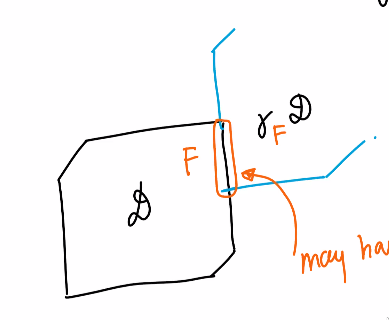
\includegraphics[scale=0.5]{fd_domain.png} \caption{Subdivision of facet}%
\label{fig:fd_domain} \end{figure} In the globally finite case, we obtain
$\gamma_{F_i} \in \Gamma$. These generate $\Gamma$ and the relations are as
follows: Note that $F' \coloneqq \gamma_F^{-1}(F)$ is a facet of $\mc{D}$. It
is also easy to see that $\gamma_{F'} = \gamma_F^{-1}$. In the case of a
reflection group, then $F = F'$ and $\Gamma_F^2 = 1$. In other words,
$\qty{\gamma_F}$ is a symmetric set of generators. We also have more
complicated relations coming from codimension $2$ strata. If the fixed
hyperplanes of $r_1, r_2$ have angle $\frac{pi}Pm$, then $r_1 r_2$ is rotation
by $2 \theta$, so we obtain the relation ${(r_1 r_2)}^m = 1$. In fact, if we
have the square lattice, then $\gamma_1 \gamma_2 = \gamma_2 \gamma_1$.

\begin{thm} The relations above are all relations between the $\gamma_F$. This
    means that \[ \Gamma = \ev{\gamma_F \mid \text{above relations}}. \]
\end{thm}

\begin{proof} Consider the exact sequence $1 \to \ker \to \wtl{\Gamma} =
    \ev{\Gamma_F \mid \text{relations}} \to \Gamma \to 1$. Now consider \[ M
    \setminus ( \text{codim}\geq 3 ) = \bigcup_{\gamma \in \Gamma}
\gamma(\mc{D} \setminus \text{codim} \geq 3). \] But now we have a covering \[
\bigcup_{\gamma \in \wtl{\Gamma}} (\gamma, \mc{D} \setminus \text{codim}\geq 3)
/ \text{relations} \to M \setminus \text{codim}\geq 3. \] However, $M \setminus
\text{codim }\geq 3$ is $1$-connected, so this covering is an isomorphism.
\end{proof}

Therefore it remains to classify possible $\mc{D}$. First, however, we will
consider a very classical example.

\begin{exm} Consider a triangle with angles $\frac{\pi}{m_{12}},
    \frac{\pi}{m_{13}}, \frac{\pi}{m_{23}}$.  Then we can consider the discrete
    reflection group $\Gamma = \ev{s_1, s_2, s_3 \mid s_i^2 = 1, {(s_i
    s_j)}^{m_{ij}} = 1}$. We have the following cases for where the triangle
    lives: \[ \frac{1}{m_{12}} + \frac{1}{m_{13}} + \frac{1}{m_{23}}
        \begin{cases} > 1 & S^2 \\ = 1 & \R^2 \\ < 1 & \H^2.  \end{cases} \]
        Thus in the first case $\Gamma$ is finite, in the second case it has
        polynomial growth, and in the final case it has exponential growth. To
        define the growth, we need to consider the length function on $\Gamma$.
        Here, we count the number of hyperplanes separating $\mc{D}, \gamma
        \mc{D}$, and this is the \textit{length} $\ell(\gamma)$, which is also
        the length of the shortest $\gamma = s_{i_1} \cdots s_{i_{\ell}}$. Some
        nice properties are that $\ell(\gamma) = \ell(\gamma^{-1})$ and that
        $\ell(\gamma s_i) = \ell(s_i \gamma) = \ell(\gamma) \pm 1$. Then we
        consider the function that takes $x$ to the number of words with length
        less than $x$, and consider the growth of this function.

    There are finitely many solutions to $\frac{1}{m_{12}} + \frac{1}{m_{23}} +
\frac{1}{m_{12}} \geq 1$, and these correspond to platonic solids (spherical)
or regular tesselations of the plane (Euclidean).  \end{exm}

Now we are ready to classify discrete reflection groups acting on $S^n$ or
$\R^n$. We can embed $S^n \subset \R^{n+1}$, so the two cases are really the
same. We want to impose that the normal vectors to the bounding hyperplanes
span ${(\R^n)}^*$. We also assume that there is no partition of the normal
vectors into two mutually perpendicular sets. We will carry out the
classification using the connection to complex semisimple Lie algebras (or
compact semisimple real Lie algebras). Consider the outer normals $e_i$ and
consider the \textit{Coxeter} matrix ${(e_i, e_j)}_{ij}$. Now we know \[ Q =
    (e_i, e_j) = \begin{cases} 1 & i = j \\ - \cos \qty(\frac{\pi}{m_{ij}}) & i
    \neq j \end{cases}. \] Because this is a Gram matrix, it is positive
    semidefinite. Also, the diagonal emenets are all positive and all
    off-diagonal elements are nonpositive. 

\begin{lem} Together with indecomposability, the two properties imply that
    either the $e_i$ are linearly independent (in which case $\mc{D}$ is a cone
    over a tetrahedron, which is the image of $\R_{\geq 0}^n$ under a linear
    map) or that $\ker Q = \R \cdot v$, where $v$ has all positive coordinates.
\end{lem}

In the first case, $\mc{D}$ is the cone over a simplex and $\Gamma$ is finite.
In the second case, $\mc{D}$ is a simplex, so it is the image of $\qty{x_i \geq
0 \mid \sum x_i = 1}$. In this case, we obtain an irreducible reflection group
in $\mr{Iso}(\R^n)$.

\begin{proof} Consider the matrix $Q$ as a quadratic form. Then the kernal
    $\ker Q = \qty{v \mid Q(v,v) = 0}$. For $v \in (v_1, \ldots, v_n)$, denote
    $\abs{v} = (\abs{v_1}, \ldots, \abs{v_n})$. Thus $Q(\abs{v}, \abs{v}) \leq
    Q(v,v)$. Thus if $Q(v,v) = 0$, we also have $Q(\abs{v}, \abs{v}) = 0$. Now
    suppose that some $v_i = 0$ and $Qv = 0$. Then ${(Qv)}_i = \sum_{j \neq i}
    q_{ij} v_j$. If there exist $i \neq j$ such that $q_{ij} \neq 0$, then
    $Q(\abs{v}, \abs{v}) < Q(v,v)$. This is impossible if $Q$ is
    indecomposable, so no $v_i$ can vanish for $v \in \ker Q$. Thus $\dim_{\R}
    \ker \leq 1$. Moreover, the kernel is closed under $v \to \abs{v}$, so it
    must be spanned by a vector with $v_i > 0$.  \end{proof}

This implies that the classification of reflection groups in $S^n, \R^n$ is the
same as the classification of indecomposable positive-semidefinite Coxeter
matrices. This is explicit and fun, and involves solving inequalities. 

Now let $\mf{k} = \Lie(K)$ for a compact group $K$ with maximal torus $T$. Then
write $\mf{g} = \mf{k} \otimes_{\R} \C$ and $\mf{t} = \Lie(T) \otimes_{\R} \C$.
Then we have a decomposition \[ \mf{g} = \mf{t} \oplus \bigoplus_{\alpha \in
\mr{char}(T)} \mf{g}_{\alpha}, \] and we know $\mf{g}_{\alpha}$ is
$1$-dimensional if and only if $\alpha$ is a root. Next, consider $e_{\alpha}
\in \mf{g}_{\alpha}, f_{\alpha} \in \mf{g}_{-\alpha}$. Then we write
$h_{\alpha} = [e_{\alpha}, f_{\alpha}] \in \mf{t}$, and this is unique. Then we
have $(h_{\alpha}, h) = \alpha(h)$ and $[h_{\alpha}, e_{\alpha}] = 2
e_{\alpha}$ and $[h_{\alpha}, f_{\alpha}] = -2 e_{\alpha}$. Therefore we have
an embedding ${\mf{sl}(2)}_{\alpha} \subset \mf{g}$, so an ${SL(2)}_{\alpha}
\subset G$. Next, consider the map \[ \beta \mapsto \beta - \frac{2(\alpha,
\beta)}{(\alpha, \alpha)} \alpha = s_{\alpha}(\beta). \] We need
$\frac{2(\alpha,\beta)}{(\alpha, \alpha)} \in \Z$ so that $s_{\alpha}(\beta)$
is in the lattice spanned by the roots. The reflections in the roots $\alpha$
generate a finite group $W$ of reflections, which also preserves the root
lattice. Now we may consider the Cartan matrix $\qty(2
\frac{(\alpha_i,\alpha_j)}{(\alpha_i, \alpha_i)})$. This is an integer matrix
with $2$ on the diagonal and nonpositive off diagonal entries. The Cartan
matrix must be positive definite.

Now each reflecting hyperplane is the zero set of a linear function (which is a
root). Now we can choose a fundamental domain, and this gives us a partition of
roots into positive and negative roots. After reflection by some $s_i$, if
$\beta \neq \alpha_i$ is a positive root, then $\beta - \alpha_i$ is still
positive after $\alpha_i$. Therefore every positive root has a sum of the form
$\beta = \sum m_i \alpha_i$, where the $\alpha_i$ are the simple positive roots
(corresponding the the faces). Moreover, this expression is unique (because the
simple roots are independent as affine linear functions).

Now recall that for a semisimple Lie algebra $\mf{g}$, we have \[ \mf{g} =
\mf{h} \oplus \bigoplus_{\alpha} \mf{g}_{\alpha}, \] where $\alpha$ ranges over
the roots. We know that $[h,e_{\alpha}] = \alpha(h) e_{\alpha}$, that
$[\mf{g}_{\alpha}, \mf{g}_{\beta}]$, that $\dim_{\C} \mf{g}_{\alpha} = 1$, and
that $\mf{g}_{\alpha} \perp \mf{g}_{\beta}$ if $\alpha + \beta \neq 0$. Also,
there exist $e_{\pm \alpha} \in \mf{g}_{\pm \alpha}$ such that $(e_{\alpha},
e_{-\alpha}) = 1$. If we write $h_{\alpha} \coloneqq [e_{\alpha},
e_{-\alpha}]$, then $(h_{\alpha}, h) = \alpha(h)$. Now our goal is go from root
systems to Lie algebras.

Because every root is either positive or negative, and every positive root can
be written uniquely as a sum of simple roots, we can write \[ \mf{g} = \mf{h}
\oplus \mf{n}_+ \oplus \mf{n}_- \qquad \mf{n}_{\pm} = \bigoplus_{\alpha > 0}
\mf{g}_{\pm \alpha}. \] Note that if $\mf{g}$ is finite-dimensional, then
$\mf{n}_+$ is nilpotent.

\begin{prop} The nilpotent Lie algebra $\mf{n}_+$ is generated by $e_i \colon
e_{\alpha_i}$, where $\qty{\alpha_1, \ldots, \alpha_r}$ are the simple positive
roots.  \end{prop}

\begin{proof} We show that if $\alpha + \beta$ is a root, then
    $[\mf{g}_{\alpha}, \mf{g}_{\beta}] = \mf{g}_{\alpha + \beta}$. Consider the
    action of ${(\mf{sl}_2)}_{\alpha}$ on $\mf{g}_{n \alpha + \beta}$. Now each
    $\mf{g}_{n_{\alpha} + \beta}$ is one-dimensional. Now recall that the
    weights of irreducible representations with respect to $h_{\alpha}$ are
    $\lambda, \lambda - 2, \ldots, 2-\lambda, -\lambda$. But now recall that
    $f_{\alpha}$ decreases the weight by $2$ and $e_{\alpha}$ increases the
    weight by $2$, and so the action of $e_{\alpha} \colon \mf{g}_{\beta} \to
    \mf{g}_{\beta + \alpha}$ is nonzero, as desired.  \end{proof}

\begin{cor} The Lie algebra $\mf{g} = \ev{h_i, e_i, f_i} / \text{relations}$,
    where $e_i = e_{\alpha_i}, f_i = e_{-\alpha_i}, h_i = h_{\alpha_i}$, where
    the $\alpha_i$ are the simple roots.

    The relations are given by \[ [h_i, e_j] = \alpha_j(h_{\alpha_i}) e_j,
    \qquad \alpha_j(h_i) = 2 \frac{(\alpha_j, \alpha_i)}{(\alpha_i, \alpha_i)}.
\] We will write $a_{ij} \coloneqq \alpha_i(h_i)$. We also have $[h_i, f_j] = -
a_{ij} f_j$ and $[e_i, f_j] = \delta_{ij} h_i$.  \end{cor}

\begin{lem}[Chevalley-Serre] For all $i,j$, we have ${\ad(e_i)}^{1-a_{ij}} e_j
= 0$.  \end{lem}

For example, for the $A_2$ root system with Cartan matrix $\begin{psmallmatrix}
2 & -1 \\ -1 & 2 \end{psmallmatrix}$, we have ${\ad(e_1)}^2 e_2 = {\ad(e_2)}^2
e_1 = 0$.

\begin{proof} Write $\square = {\ad(e_i)}^{1-a_{ij}} e_j$. We will prove that
    if $[f_k, \square] = 0$, then $\ad(\mf{g}) \square$ is invariant under
    $\mf{g}$. Then $\square$ is a lowest weight vector, so $\ad(\mf{g}) \square
    \subset \mf{n}_+$ would be a proper submodule, contracticting the
    simplicity of $\mf{g}$.

    Now we need to prove that $[f_k, \square] = 0$. This is clear for $k \neq
    i,j$, so we need to check it for $k=i$ and $k=j$. For $k=i$, we have
    weights $a_{ij}, a_{ij}+2, \ldots, -a_{ij}$ for $h_i$ (by the action of
    ${(\mf{sl}_2)}_i$ on $e_j$), so $\square$ corresponds to the weight
    $-a_{ij} + 2$, so we must have $\square = 0$ (because otherwise it would
    generate an infinite-dimensional module). Now we consider the case when
    $k=j$. Here, we have \begin{align*} [f_j, {(\ad e_i)}^{1-a_{ij}} e_j] &= -
    {(\ad e_i)}^{1-a_{ij}} h_j \\ &= {(\ad e_i)}^{-a_{ij}} [e_i, h_j] \\ &=
{(\ad e_i)}^{-a_{ij}} (-a_{ij} e_i).  \end{align*} Now if $a_{ij} < 0$, we see
$[e_i, e_i] = 0$ and if $a_{ij} = 0$, we also have vanishing.  \end{proof}

\begin{thm} For a simple Lie algebra $\mf{g}$, we have $\mf{g} = \ev{h_i, f_i,
    e_i} / \text{relations}$ with the Cartan matrix $C = (a_{ij}) = 2
    \frac{(\alpha_i, \alpha_j)}{(\alpha_j, \alpha_j)}$. Moreover, for any
    matrix $C$ such that $a_{ii} = 2$, $a_{ij} \leq 0$, and $C$ is
    symmetrizable, then the matrix $\mf{g}$ is simple and finite-dimensional if
    and only if $C$ corresponds to a finite root system.  \end{thm}

\begin{rmk} Note that the conditions that $a_{ii} = 2, a_{ij} \leq 0$, and $C$
is symmetrizable can be relaxed in principle.  \end{rmk}

\section{Kac-Moody Lie algebras}% \label{sec:kac_moody_lie_algebras}

Let $C = (a_{ij})$ be a matrix such that $a_{ii} = 2, a_{ij} \leq 0$, and
$a_{ij} = 0$ if and only if $a_{ij} = 0$. Note this is weaker than being
symmetrizable. Now we define the Lie algebra \[ \left. \wtl{\mf{g}} = \ev{e_i,
f_i, h_i} \middle/ \qty( \Vectorstack{ {[h_i, e_i] = a_{ij} e_j} {[h_j, f_j] =
-a_{ij} f_j} {[e_i, f_j] = \delta_{ij} h_i} } ) \right. . \] Now we have the
decomposition $\wtl{\mf{g}} = \mf{h} \oplus \wtl{\mf{n}}_+ \oplus
\wtl{\mf{n}}_-$, where $\wtl{\mf{n}}_+$ is the free Lie algebra generalized by
the $e_i$, whose universal enveloping algebra is a free associative algebra.
Note if $C = (2)$, then $\wtl{\mf{g}} = \mf{sl}_2$. Also, we have \[
    \wtl{\mf{n}}_+ = \bigoplus_{\alpha = \sum m_i \alpha_i \geq 0}
    \mf{g}_{\alpha}, \] so in fact all roots are already either positive or
    negative. Here, note that \[ [f_i, \mf{n}_+] \subset \C h_i \oplus
    \mf{n}_+, \] and we also know that \[ [f_1, [e_1, e_2]] = -[h_1, e_2] =
-a_{12} e_2. \] The previous argument for $\square = {\ad(e_i)}^{1-a_{ij}} e_j$
shows that it is a lowest weight vector in $\mf{n}_+$. Now we know that
$\mf{n}_+ \supseteq \ad(\wtl{\mf{g}}) \square$. More generally, we can consider
the maximal submodule of $\ad(\wtl{\mf{g}})$ (which cannot contain the $e_i$). 

\begin{defn} We define the \textit{Kac-Moody algebra} $\mf{g}_{\mr{KM}}$ to be
the quotient of $\wtl{\mf{g}}$ by the maximal submodules in $\mf{n}_+$ and
$\mf{n}_-$.  \end{defn}

\begin{thm}[Gabber-Kac] If $C$ is symmetrizable, then the maximal submodules in
$\mf{n}_+, \mf{n}_-$ are generated by the Chevalley-Serre relations.  \end{thm}

\begin{thm} If $\dim \mf{g}_{\mr{KM}} < \infty$, then $C$ corresponds to a
finite reflection group.  \end{thm}

\begin{rmk} There are even larger generalizations of this, for example
Borcherds-Kac-Moody Lie algebras and other classes of Lie algebras.  \end{rmk}

Now Chevalley-Serre tells us that for large enough $M$, ${\ad(e_i)}^M$ applied
to any generator vanishes. Thus for any $x \in \mf{g}_{\mr{KM}}$, there exists
$M = M(x)$ such that ${\ad(e_i)}^M x = {\ad(f_i)}^M x = 0$. I particular, any
$x \in \mf{g}_{\mr{KM}}$ is contained in a finite-dimensional ${\mf{sl}(2)}_i =
\ev{e_i, f_i, h_i}$-module.

By definition, a $\mf{g}_{\mr{KM}}$-module is \textit{integrable} if for all
${\mf{sl}(2)}_i$, the module decomposes as a sum of finite-dimensional modules.
Thus, in this language, the adjoint representation of $\mf{g}_{\mr{KM}}$ is
integrable. Now we can integrate each ${\mf{sl}(2)}_i$-module to ${SL(2)}_i$,
and the matrix $\begin{psmallmatrix} 0 & -1 \\ 1 & 0 \end{psmallmatrix}$ acts
by reflection $r_i$. Then we see that \[ r_i(\lambda) = \lambda - \lambda(h_i)
\alpha_i, \] and the $r_i$ generate the Weyl group of $\mf{g}_{\mr{KM}}$. In
particular, it permutes the set of roots.

Recall that when we had an invariant quadratic form, we had the identity \[
(h_i, h_j) = (h_i, [e_j, f_j]) = ([h_i, e_j], f_j) = a_{ij} (e_j, f_j). \]
Therefore there exists an invariant quadratic form if and only if there exists
a diagonal $D$ such that $CD$ is symmetric. Now note that $\wtl{ \mf{g} } =
\mf{h} \oplus \mf{n}_+ \oplus \mf{n}_-$, and $\mf{n}_+, \mf{n}_-$ are dual with
respect to the quadratic form. In fact, we obtain expressions of the form \[ (
    \ad(e_i) e_j, f_k ) = - (e_j, \ad(e_i) f_k). \] Now if we consider the
    ideal of relations $\mf{r}_+ \subset \mf{n}_+$, then we note that \[ (r,
    \ad(f_i) *) = - (\ad(f_i) r, *) = 0. \] Now note that any invariant
    bilinear form on $\mf{g}$ is nondegenerate because $\mf{g}^{\perp}$ is an
    ideal which does not intersect $\mf{h}$, and thus vanishes. If $a_{ii} \neq
    0$, then we can assume $a_{ii} = 2$, and therefore we have a subalgebra
    ${\mf{sl}(2)}_i = \ev{e_i, f_i, h_i}$, then for $j \neq i$, $e_j$ is the
    lowest weight vector for ${\mf{sl}(2)}_i$ with weight $a_{ij}$. If $a_{ij}
    \in 0,-1,-2,\ldots$, then it is possible that the ${\mf{sl}(2)}_i$-module
    is finite-dimensional. Kac-Moody theory is about \textit{integrable
    modules}. Also, recall that ${\ad(e_i)}^{1-a_{ij}} e_j = 0 \in \mf{g}$, and
    by Gabber-Kac this is the complete list of relations. Also recall the
    adjoint representation is integrable.

\begin{exm} Consider $C = \begin{psmallmatrix} 2 & a_{12} \\ a_{21} & 2
\end{psmallmatrix}$. Note that if we want $\det C > 0$, we can only have
$(a_{12}, a_{21}) = (-1,-1), (-2,-1), (-3,-1)$. Now the three cases correspond
to the Lie algebras $\mf{sl}_3, \mf{sp}(4) = \mf{so}(5), G_2$. In the case
where $\det C = 0$, or $(a_{12}, a_{21}) = (-2,-2), (-4,-1)$, then we need to
enlarge $\mf{h}$ to have $\alpha_j(h_i) = a_{ij}$. The extra elements in
$\mf{h}$ will be central, and we will need to consider a central extension of
$\mf{sl}(2) \otimes \C[t^{\pm 1}]$. Here, we will have \[ e_1 = \begin{pmatrix}
    0 & 1 \\ 0 & 0 \end{pmatrix}, \qquad e_2 = \begin{pmatrix} 0 & 0 \\ t & 0
    \end{pmatrix}, \qquad f_1 = \begin{pmatrix} 0 & 0 \\ 1 & 0 \end{pmatrix},
    \qquad f_2 = \begin{pmatrix} 0 & t^{-1} \\ 0 & 0 \end{pmatrix}. \] Now we
    have \[ \mf{h} = \C \begin{psmallmatrix} 1 & 0 \\ 0 & -1 \end{psmallmatrix}
\oplus \C \cdot \text{central} \oplus \C \cdot t \dv{t}. \] These are called
affine Lie algebras, and these correspond to reflection groups in $\R^n$. Now
consider the case when $\det C < 0$. This is much more complex, and suppose
$a_{12} = a_{21} = -m$, where $m>4$. Then the quadratic form $\norm{(x,y)}^2 =
2x^2 - 2mxy + 2y^2$ has signature $(1,-1)$. Now after we kill the Serre
relations, we have our Weyl group $W = \ev{r_1, r_2}$, where \[ r_1 = \mqty(-1
& m \\ 0 & 1), \qquad r_2 = \mqty(1 & 0 \\ m & -1). \] It is easy to see that
$r_2 (1,0) = (1,m), r_2 (0,1) = (0,-1), r_1(0,1) = (m,1), r_1(1,0) = (-1,0)$.
Now the vectors with $\norm{-}^2 = 2$ form a hyperbola, and it is easy to see
that $r_1, r_2$ are translations on the hyperbola. Note that these are
solutions to $x^2 - mxy + y^2 = 1$ and are units in $\Q(\sqrt{m^2-4})$. Also,
note that \[ \frac{m+\sqrt{m^2-4}}{2} = m - 1 + \frac{1}{1 + \frac{1}{m-2 +
\cdots}} \] is periodic and the coefficients are $1, m-2$. 

    The fact that there are no roots of $\wtl{\mf{g}}$ in $\Z_{\geq 0} \times
\Z_{\leq 0} \setminus \qty{(0,1), (1,0), (0,0)}$ and the $W$-action implies
that there are no roots with $\norm{-}^2 > 2$. Now for $\beta = m_1 \alpha_1 +
m_2 \alpha_2$, we would like to minimize the height $m_1 + m_2$. Now if $(r_i,
\beta) = \beta - (\alpha_i, \beta) \alpha_i$, then we can decrease the height
unless $\beta = \alpha_i$. Now in every $W$-orbit of a root $\beta$, either
there is a simple root $\alpha_i$, so $\norm{\beta}^2 = 2$, or there is a root
with $(\beta, \alpha_i) > 0$ for all $i$. Now roots are either real (which
means $\dim \mf{g}_{\beta} = 1$) or imaginary (which implies exponential growth
in the cone bounded by lines of slope $m/2, 2/m$). In general, if the signature
of our matrix $(n-1,1)$, there is a similar picture, where we have a light cone
(notation stolen from physics, all hyperboloids will asymptotically converge to
this), and inside we have the funramental domain. Unfortunately, there is only
a compact fundamental domain in low dimension, so the theory fails in high
dimension. If the signature is worse, then the theory gets worse. However,
every root is either real or belongs to the orbit of a fundamental domain
(which is the set of vectors such that $(\beta, \alpha_i) \leq 0$ for all but
finitely many roots).  \end{exm}

It should be clear that $\dim \mf{g} < \infty$ if and only if $C > 0$. This
explains why we end up with infinite-dimensional Lie algebras when we attempt
classification.

\section{Integrable representations of Kac-Moody Lie algebras}%
\label{sec:integrable_representations_of_kac_moody_lie_algebras}

Let $\mf{g} = \mf{h} \oplus \mf{n}_+ \oplus \mf{n}_-$ be a symmetrizable
Kac-Moody Lie algebra and $C = (a_{ij})$ be the Cartan matrix. Then the Weyl
group $W = \ev{r_i}$ acts on $\mf{h}, \mf{h}^*$.

Now if $M$ is a module and $v \in M$, by definition $v$ is a \textit{highest
weight vector} if $h_i v = \lambda(h_i) v$ for some $\lambda \in \mf{h}^*$ and
$e_i v = 0$ for all $i$. Some examples of highest weight modules are
\textit{Verma modules} $M_{\lambda}$, which is the free module generated by a
highest weight vector $v_{\lambda}$. Equivalently, we can write \[ M_{\lambda}
= \mc{U}(\mf{g}) \otimes_{\mc{U}(\mf{h} \oplus \mf{n}_+)} \C_{\lambda}. \] This
is not even close to being integrable (just note we can act infinitely many
times by $f_i$). To make $M_{\lambda}$ integrable, we need $\lambda(h_i) =
0,1,\ldots$ to be a nonnegative integer and $f_i^{\lambda(h_i)+1} v = 0$. This
gives us a candidate for an irreducible integrable module $L_{\lambda}$ with
highest weight\footnote{Allegedly there is a physical interpretation for the
existence of a highest weight vector.} $\lambda$. We will see later that this
is indeed irreducible by the classification of irreducible finite-dimensional
modules. We will also compute the character using the Weyl-Kac formula.

We will now consider the Casimir element. First suppose that $\dim \mf{g} <
\infty$ and let $x_i, y_i$ be dual bases for the Killing form $(-,-)$. Then the
Casimir element is \[ C = \sum x_i y_i \in \mc{U}(\mf{g}). \] Now because
$\mf{g}_{\alpha}$ is dual to $\mf{g}_{-\alpha}$, we have \[ C = \sum h_i^2 +
    \sum_{\alpha > 0} (e_{\alpha} f_{\alpha} + f_{\alpha} e_{\alpha}). \] This
    acts by a scalar in $M_{\lambda}$ because it commutes with all $f_i$, and
    so \[ C v = \sum { \lambda(h_i) }^2 + \sum_{\alpha > 0}
    \lambda(h_{\alpha}). \] For any $h \in \mf{h}$, we have $(h, h_{\alpha}) =
    \alpha(h) (e_{\alpha}, f_{\alpha})$. Now consider \[ \rho = \frac{1}{2}
    \sum_{\alpha >0} \alpha \in \mf{h}^*. \]

\begin{lem} For all $r$, $r_i(\rho) = \rho - \alpha_i$. In other words,
$\rho(h_i) = 1$.  \end{lem}

\begin{proof} Note that $r_i$ permutes the set of positive roots distinct from
$\alpha_i$. Therefore $r_i(\alpha_i) = -\alpha_i$, and the desired result
follows by splitting the expression for $\rho$.  \end{proof}

\begin{rmk} Some analog of this also makes sense if $\dim \mf{g} = \infty$.
\end{rmk}

We can take any other function of the set $\qty{\alpha > 0 \mid \alpha \neq
\alpha_i}$, such as $x \mapsto 1-e^{-x}$. Then the product \[ e^{\rho}
\prod_{\alpha > 0} (1-e^{-\alpha}) \] is a Laurent series in $e^{-\alpha_i}$
which is often analytically convergent. Under the action of $r_i$, we obtain \[
e^{\rho-\alpha_i} (1-e^{\alpha_i}) \prod_{\alpha \neq \alpha_i} (1-e^{-\alpha})
= -e^{-\rho} \prod (1-e^{-\alpha}). \] Therefore this product is
$W$-anti-invariant. Note that the product $\prod_{\alpha >0}
\frac{1}{1-e^{-\alpha}}$ is the character of $h^{\mf{h}}$ acting on
$\mc{U}(\mf{n}_-)$. Here, the operators $1, f_{\alpha}, \ldots$ have weight
$1,e^{-\alpha}. e^{-2\alpha},\ldots$, and taking the sum, we obtain the
expression. Therefore, the character of a Verma module is \[
\frac{e^{\lambda}}{\prod_{\alpha > 0} (1-e^{-\alpha})}. \]

\begin{thm}[Weyl-Kac] The character of the integrable representation
    $L_{\lambda}$ is given by \[ \sum_{w \in W} w \cdot
    \qty(\frac{e^{\lambda}}{\prod_{\alpha > 0} (1-e^{-\alpha})}) =
\frac{1}{\prod_{\alpha > 0}(1-e^{-\alpha})} \sum_w {(-1)}^w e^{w(\lambda +
\rho) - \rho}. \] \end{thm}

Returning to the Casimir element, we now write \[ C = \sum h_i h^i +
\sum_{\alpha > 0} h_{\alpha} + 2 \sum_{\alpha > 0} e_{\alpha} f_{\alpha}. \]
For infinite-dimensional modules with highest weight, this expression makes
sense because the final term in the sum is locally finite. Here, $h^i$ is the
dual basis to the $h_i$. This still commutes with the $f_i$. Therefore $C$ acts
on $M_{\lambda}$ by $(\lambda, \lambda) + 2 (\lambda, \rho) = (\lambda + \rho,
\lambda + \rho) - (\rho, \rho)$.

To prove this, consider the exact sequence \[ 0 \to M \to M_{\lambda} \to
L_{\lambda} \to 0. \] Here, $M$ is some highest-weight module, so it has a
surjection from $\bigoplus M_{\mu_i}$. Thus there exists a resolution of
$L_{\lambda}$ by Verma modules of the form \[ \cdots \to \bigoplus M_{\nu_j}
\to \bigoplus M_{\mu_i} \to M_{\lambda} \to L_{\lambda} \to 0. \] By the action
of the Casimir element, we have $\norm{\mu_i + \rho}^2 = \norm{\lambda +
\rho}^2$. In addition, the character of $L_{\lambda}$ is $W$-invariant by
integrability. Together, we obtain that the character of $L_{\lambda}$ is a sum
of the form \[ \sum_{\mu} c_{\mu} \mr{char}(M_{\mu}), \] where $\lambda - \mu$
is either a sum of positive roots or zero, $c_{\lambda} = 1$, $\norm{\mu +
\rho}^2 = \norm{\lambda + \rho}^2$, $c_{\mu}$ is anti-invariant under the
action of $W$ by $w \cdot \mu = w(\mu +\rho)-\rho$.

\begin{lem} Every $\mu$ such that $\lambda - \mu$ is a sum of roots can be
brought by the $W \cdot$ action to the positive cone (where $(\mu,\alpha_i)
\geq 0$). The positive cone is also called the dominant cone.  \end{lem}

\begin{proof} Choose $w$ such that in the expression $\lambda + \rho - w(\mu +
\rho) = \sum m_i \alpha_i$, $\sum m_i$ is minimal. If $(\mu, \alpha_i) < 0$,
then we can apply $r_i$ and decrease $m_i$.  \end{proof}

\begin{lem} If $(\lambda, \alpha_i) > 0, (\mu, \alpha_i) \geq 0$, $\lambda \geq
\mu$, and $(\lambda, \lambda) = (\mu, mu)$, then $\lambda = \mu$.  \end{lem}

Proof of this result is left as an exercise to the reader.

As a consequence, we have: \begin{enumerate} \item If $c_{\mu} \neq 0$, then
    the intersection of $W \cdot \mu$ with the dominant cone is simply
    $\lambda$, and thus $c_{\mu} {(-1)}^w \delta_{W \cdot \lambda}$.  \item In
    the exact sequence $\bigoplus \mc{U}(\mf{n}_-) f_i^{\lambda(h_i)+1} v \to
    M_{\lambda} \to \mr{coker} \to 0$, the first term is simply
    $\bigoplus_{r_i} M_{r_i \cdot \lambda}$. Now the cokernel is irreducible
    because it is integrable and therefore there is no room for other singular
    vectors. In fact, this can be continued to a Bernstein-Gelfand-Gelfand
    resolution of $L_{\lambda}$ by \[ \cdots \to \bigoplus_{\ell(w)=k} M_{w
\cdot \lambda} \to \cdots \] \end{enumerate}

As a corollary of Weyl-Kac we obtain \begin{cor}[Denominator identity] Apply
    the formula to $L_0 = \C$ to obtain \[ 1 = \frac{e^{-\rho}}{\prod_{\alpha >
        0} (1-e^{-\alpha})} \sum_w {(-1)}^w e^{w \rho} \] and rearrange to
        obtain \[ \sum_w {(-1)}^w e^{w \rho} = e^{\rho} \prod_{\alpha > 0}
        (1-e^{-\alpha}). \] \end{cor}

For example, when $\mf{g} = \mf{sl}(n)$, the positive roots are of the form
$(0, 1, \ldots, -1, 0)$, so $e^{\alpha} = \frac{x_i}{x_j}$. Then we have $\rho
= ((n-1)/2, \ldots, (1-n)/2)$, and therefore we have \[ x^{\ldots} \prod_{i >
j} \qty(1-\frac{x_j}{x_i}) = \sum_{s \in S_n} {(-1)}^s s(x^{\ldots}). \] This
has the more familiar form \[ \prod_{i > j} (x_i - x_j) = \sum_{s\in S_n}
{(-1)}^s s \cdot (x_1^{n-1} \cdots x_n^0). \] For $\wh{\mf{sl}}_2$, this gives
us the \textit{Jacobi triple product identity} for theta functions \[
\vartheta(x;q) = \sum_n {(-1)}^n x^n q^{n^2/2} = \prod_{n > 0} (1-q^n)
\prod_{n>0} (1-xq^n) \prod_{n \geq 0} (1-x^{-1} q^n). \]

\section{Affine Lie Algebras}% \label{sec:affine_lie_algebras}

Let $\Gamma = \ev{r_i}$ be a group of isometries in $\R^n$. For example, if
$r_1, r_2, r_3$ are reflections along the sides of an equilateral triangle, we
have the $\wh{A}_2$ group. Now isometries of $\R^n$ embed in isometries of
$\H^{n+1}$ because we can embed $\R^n$ as a horocycle. Now consider the group
$\wh{A}_1$ generated by $r_1, r_2$ with $r_1 r_2$ of infinite order. If we
consider spheres $S^n$ in $\H^{n+1}$, we have an action of $SO(n)$ on $S^n$
which commutes with the action of $SO(n,1)$ on $\H^{n+1}$. Note that $SO(n)$
stabilizes a vector of negative norm. In the limit as the radius approaches
$\infty$, the curvature approaches $0$, so we obtain $\R^n$.

Now the semidirect product $SO(n-1) \ltimes \R^n$ stabilizes a null vector, so
it acts on $\R^n \subset \H^{n+1}$. Now if we fix that $SO(n,1)$ preserves the
form $x_0 x_n + x_1^2 + \cdots + x_{n-1}^2$, then if we consider the light cone
where $\norm{x'}^2 + x_0 x_n = 0$, then our isometry group acts in a way such
that orbits are like parabolas. In the case of $\wh{A}_1$, the orbit of a
single point in $\R^1$ will lie on a parabola when we embed in $\R^{2,1}$.

Now our reflection group $\wh{A}_1$ could have Cartan matrix
$\begin{psmallmatrix} 2 & -2 \\ -2 & 2 \end{psmallmatrix}$ or
$\begin{psmallmatrix} 2 & -4 \\ -1 & 2 \end{psmallmatrix}$. The first
corresponds to a central extension $\wh{\mf{sl}}(2)$ of $\mf{sl}(2) \otimes
\C[t,t^{-1}]$ while the second corresponds to a twisted loop algebra. Here, if
$\mf{g}$ is a Lie algebra and $\sigma$ is an automorphism of order $m$, then we
may consider the subalgebra \[ \qty{f(t) \mid f(t \zeta_m) = \sigma f(t) }
\subset \mf{g}[t,t^{-1}]. \] For example, note that $\mf{sl}(2)[t^{\pm 1}]$ is
generated by the matrices \[ e_1 = \mqty(0 & 1 \\ 0 & 1), f_1 = \mqty(0 & 0 \\
    1 & 0), e_0 = \mqty(0 & 0 \\ t & 0), f_0 = \mqty(0 & t^{-1} \\ 0 & 0). \]
    Then $[e_1, f_1] = h_1 = -[e_0, f_0]$. If we define $h_0 \coloneqq [e_0,
    f_0]$, then for $C = \begin{psmallmatrix} 2 & -2 \\ -2 & 2
    \end{psmallmatrix}$, $h_0 + h_1$ is contained in the kernel of the map \[ 0
\to \C(h_0 + h_1) \to \ev{h_1, e_0, f_0, h_1, f_1, e_1} \mapsto \mf{sl}(2)
[t^{\pm 1}] \to 0. \] Now note that if we set $\deg e_0 = (1,0), \deg e_1 =
(0,1)$, then the Lie algebra $\ev{h_0, e_0, f_0, h_1, f_1, e_1}$ is graded by
$\Z^2$. Because $C$ is degenerate, only one of these two gradings is internal.
To restore the grading, we introduce the element $D \coloneqq t \dv{t}$, where
$D e_0 = e_0$ and $D f_0 = -f_0$. Now we set \[ \mf{g} = \mf{h} \oplus
    \bigoplus_{\alpha > 0} \mf{g}_{\alpha}, \qquad C' = \mqty(2 & -2 \\ -2 & 2
    \\ 1 & 0) \] where we set $h_2 = D$. Now we have a map \[ 0 \to \C(h_0 +
h_1) \to \ev{h_0, h_1, h_2, e_0, f_0, e_1, f_1} \to \C t \dv{t} \ltimes
\mf{sl}(2)[t^{\pm 1}] \to 0. \] Now because there are three simple roots, the
matrix of the invariant bilinear form is \[ \mqty(2 & -2 & 1 \\ -2 & 2 & 0 \\ 1
& 0 & 0), \] and this has signature $(2,1)$. In the basis of $C=(h_0+h_1), h_1,
D$, this takes the form \[ \mqty( & & 1 \\ & 2 & \\ 1 & & ), \] which is
precisely of the form $x_0 x_{n+1} + x_1^2 + \cdots + x_n^2$.

Now we would like to describe the central extension in terms of matrices. Here,
we have \[ [e_0, f_0] = h_0 = C - h_1 = \qty[ \begin{psmallmatrix} 0 & 0 \\ t &
    0 \end{psmallmatrix}, \begin{psmallmatrix} 0 & t^{-1} \\ 0 & 0
\end{psmallmatrix}] + C \cdot 1, \] then we can write $1 = \Res \tr P'(t) Q(t)
    = \Res \qty( \dv{t} P(t), Q(t) )$ if we set $e_1 = P(t), f_1 = Q(t)$. Using
    integration by parts, this is skew-symmetric. Now we have \[ \mf{g} =
    \mf{h} \oplus \bigoplus_{n \in \Z} \C \mqty(0 & t^n \\ 0 & 0) \oplus
\bigoplus_{n \in \Z} \C \mqty(0 & 0 \\ t^n & 0) \oplus \bigoplus_{n \neq 0} \C
\mqty( \dmat{t^n,-t^n} ). \] Now the eigenvalues of $(C, h_1, D)$ on each
factor are $(0, 2,n), (0, -2, n), (0, 0,n)$. The values $x+n (n \geq 0), -x+n
(n \geq 1), n (n \geq 1)$ are positive for $x \in (0,1)$. Now if we define \[
\Delta \coloneqq \prod_{\alpha > 0} (1-e^{-\alpha}), \] then if we set
$\exp(0,0,-1) = q, \exp(0,1,0) = x$, we obtain \[ \Delta = (1-x^{-1})
\prod_{n>0} (1-q^n x^{-1}) (1-q^n) (1-q^n x). \] This is simply the genus $1$
theta function $\vartheta(x)$, which has the property that $\vartheta(1) = 0$
and that \[ \vartheta(qx) = (1-q^{-1}x^{-1}) \prod_{n>0}
(1-q^{n-1}x^{-1})(1-q^n)(1-q^{n+1}x) = \vartheta(x) \frac{1-q^{-1}x^{-1}}{1-qx}
= -q^{-1}x^{-1} \vartheta(x). \] Therefore $\vartheta$ is a section of a degree
$1$ line bundle over $\E \coloneqq \C^{\times} / q^{\Z}$. Note that $\Delta$
converges analytically if $\abs{q} < 1$. Because $-q^{-1} x^{-1}$ is
invertible, we may use it as a clutching function. By Riemann-Roch, $\vartheta$
only has a single zero at $x=1$.

Another way to write solutions of the equation $\vartheta(qx) = -q^{-1}x^{-1}
\vartheta(x)$ is using the form $\sum x^m q^{m^2/2}$. Here we want to think of
$\frac{m^2}{2}$ as $\binom{m}{2}$, so if we apply $x \mapsto qx$, we have \[
\sum x^m q^{\frac{m(m-1)}{2}} \mapsto \sum_m x^m q^{\frac{m(m+1)}{2}} = x^{-1}
\sum_m x^m q^{\frac{m(m-1)}{2}}, \] and thus we have $\wtl{\vartheta}(qx) =
x^{-1} \wtl(\vartheta)(x)$. Therefore $\vartheta(x) \approx \mr{const}
\wtl{\vartheta}(-qx)$, and thus everything is unique up to a multiple section
of a line bundle on $\E$. Classically, this is the Jacobi product formula. As a
sum, we really have the sum in the Weyl-Kac formula, because \[ \Delta =
\prod_{\substack{\alpha>0 \\ n \geq 0}} (1-q^n x^{\alpha})
\prod_{\substack{\alpha<0 \\ n>0}} (1-q^n x^{\alpha}) \prod_{n > 0}
{(1-q^n)}^{\rank \mf{g}}. \] This also satisfies some $q$-difference equation,
so is a section of a Line bundle of $\E^{\rank \mf{g}}$. In general, we have \[
\Delta = \sum_{W_{\mr{finite}} \ltimes \Z^r} {(-1)}^{\mr{sign}}
q^{\text{quadratic}} x^{\text{something}}, \] and this can be rewritten as an
expression in the characters of $\mf{g}_{\text{finite}}$ is we sum over $W$
first and as a theta function if we sum over the lattice first.




\end{document}
